%*************************************************************************
%	PLANTILLA PARA LA EDICIÓN DE PROYECTOS FIN DE CARRERA
%	Departamento de Teoría de la Señal y Comunicaciones
%	Universidad de Alcalá
%*************************************************************************

%******************
%Tipo de documento
%******************
%Descomentar la opción que corresponda:
%Versión durante la revisión (incluye números de línea)
\documentclass[12pt,twoside]{book}
\usepackage{lineno}
\linenumbers
%Versión final para imprimir a doble cara
%\documentclass[12pt,twoside]{book}
%Versión final para imprimir a una sola cara
%\documentclass[12pt,oneside]{book}

%********************
%Paquetes a utilizar
%********************

\usepackage[square,numbers]{natbib}
\usepackage[T1]{fontenc}
\usepackage[spanish]{babel}
\usepackage{verbatim}
\usepackage{amssymb}
\usepackage{amsmath}
\usepackage{fancyhdr}
\usepackage{graphicx}
\usepackage{multicol}
\usepackage{makeidx}
%\usepackage[bf,SL,BF]{subfigure}
\usepackage{subcaption}
\usepackage{caption}
\usepackage[utf8]{inputenc}
\usepackage{color}
\usepackage{multirow}
\usepackage{float}
\usepackage[printonlyused]{acronym}


\usepackage[pagebackref=true,breaklinks=true,letterpaper=true,colorlinks,bookmarks=false]{hyperref}
%No incluir paquetes depués de este.

%*************
%Definiciones
%*************
\deactivatetilden 
\addto\captionsspanish{\def\tablename{Tabla}\def\listtablename{Lista
de tablas}\def\listfigurename{Lista de figuras}}
%Cambios en los márgenes
\renewcommand{\baselinestretch}{1.1}

\setlength{\oddsidemargin}{0.4cm}
\setlength{\evensidemargin}{-0.4cm} \setlength{\headsep}{0.75cm}
\setlength{\textheight}{23cm} \setlength{\textwidth}{16cm}
\setlength{\topmargin}{-0.25cm}\flushbottom



%***************
%Título del TFC
%***************
\title{Sistema de adaptación inteligente de la velocidad para vehículos basado en IA y visión por computador}

%****************
%Autor
%****************
\author{Sergio Sastre Arrojo}

%Prepara el índice
\makeindex



%***********************
%Comienzo del documento
%***********************
\begin{document}
\setcounter{tocdepth}{4} \setcounter{secnumdepth}{3}

\frontmatter

%Incluimos fichero previo.tex -> genera la hoja de calificación y la portada
\begin{titlepage}
%**********************************************************
%GENERA LA HOJA OFICIAL DE CALIFICACIÓN PARA PROYECTOS FIN DE CARRERA
%SEGÚN EL FORMATO DE LA UNIVERSIDAD DE ALCALÁ Y DEL DEPAR-
%TAMENTO DE TEORÍA DE LA SEÑAL Y COMUNICACIONES.
%**********************************************************

\begin{center}
\LARGE \textsc{Universidad de Alcalá}\\
\vspace{0.5cm}

%Nombre de la escuela-> seleccione el que corresponda.
\textbf{Escuela Politécnica Superior}\\
%\textbf{Escuela Técnica Superior de Ingeniería Informática}\\

%Titulación -> escriba su titulación
Grado en Ingeniería Telemática
\end{center}

\vspace{0.5cm}

\begin{center}
%Para compilar con latex

\includegraphics[width=4cm]{Figuras/LogoUAH.eps}\\
%Para compilar con pdflatex
%
\includegraphics[width=4cm]{Figuras/LogoUAH.png}\\
\end{center}


\begin{center}
\vspace{1cm}

\LARGE Proyecto Fin de Carrera\\
\textbf{\Huge \textsc{{Sistema de adaptación de la velocidad para vehículos basado en IA y visión por computador}}}\\
\vspace{0.5cm}
\large Autor: Sergio Sastre Arrojo\\
Director: Roberto Javier López Sastre\\
\vspace{0.5cm}
\end{center}

\begin{flushleft}
\textbf{TRIBUNAL:}\\
\vspace{1.5cm}
\textit{Presidente: Manuel Utrilla Manso}\\
\vspace{1.5cm}
\textit{Vocal 1º: Pedro Gil Jiménez}\\
\vspace{1.5cm}
\textit{Vocal 2º: Roberto Javier López Sastre}\\
\vspace{1.5cm}
\textbf{CALIFICACIÓN:}............................................................ FECHA:.................... \\
%IMPORTANTE!
%La copia en PDF para la biblioteca, y uno de los tomos no lleva espacio para la PUBLICACIÓN!
\end{flushleft}
%Final de la hoja de calificación.

%Introduce hoja en blanco
\newpage
\thispagestyle{empty}
\hspace*{0.5cm}
\newpage


\end{titlepage}

%Prepara el título del proyecto.
\maketitle

%Introduce hoja en blanco
\newpage
\thispagestyle{empty}
\hspace*{0.5cm}
\newpage

%Incluye las dedicatorias (fichero dedicatorias.tex)
\begin{flushright}
\textit{Dedicado a mi familia, por haberme apoyado durante este largo camino.
A mis amigos, por haberme ayudado cuando más lo necesitaba.
A mis compañeros, con los que he compartido grandes momentos durante estos años de formación.
A mi tutor, por haber depositado su confianza en mí para este proyecto.
Y, en especial, a mis abuelos, por enseñarme a seguir adelante a pesar de las dificultades.}
\end{flushright}
%Introduce hoja en blanco
\newpage
\thispagestyle{empty}
\hspace*{0.5cm}
\newpage


%Incluye los agradecimientos (fichero agradecimientos.tex)
\chapter{Agradecimientos}
Gracias a todos los profesores y compañeros con los que me he cruzado y conocido durante una de las etapas más duras de mi vida, de los cuales he aprendido diferentes valores y me han enseñado cosas que, de otra forma, no hubiera aprendido. A mi familia, por criarme y educarme en la honestidad, la perseverancia, la resiliencia, y la satisfacción de un trabajo bien hecho. A mis amigos, por enseñarme el verdadero valor de la amistad al mostrarme su apoyo incondicional en situaciones tanto adversas como favorables.
%Siempre hay alguien a quien agradecerle algo, y más cuando has hecho un Proyecto Fin de Carrera (PFC).

%Introduce hoja en blanco
\newpage
\thispagestyle{empty}
\hspace*{0.5cm}
\newpage

%Inlcuimos el índice que latex genera automáticamente.
\tableofcontents
%La lista de figuras incluidas en el proyecto.
\listoffigures
%La lista de tablas.
\listoftables


%Incluye el resumen del Proyecto fin de carrera (fichero resumen.tex)
\chapter{Resumen}
\textcolor{red}{Resumen de 100 palabras MÁXIMO}\\


\vspace{0.5cm}

\textbf{Palabras clave}: cinco palabras como máximo, separadas por comas.

%Introduce hoja en blanco
\newpage
\thispagestyle{empty}
\hspace*{0.5cm}
\newpage

\chapter{Abstract}
\textcolor{red}{Resumen de 100 palabras MÁXIMO - Es OBLIGATORIO}\\

\vspace{0.5cm}

\textbf{Keywords}: cinco palabras como máximo, separadas por comas.
%Introduce hoja en blanco
\newpage
\thispagestyle{empty}
\hspace*{0.5cm}
\newpage

%Incluye el resumen Extendido del Proyecto fin de carrera (fichero resumen-extendido.tex)
\chapter{Resumen Extendido}
Debe incluir un resumen del trabajo de un máximo de 5 páginas. Resaltar aspectos fundamentales del desarrollo, los resultados más relevantes y las conclusiones.



%Incluimos lista de abreviaturas
\chapter{Glosario}

%Lista con los acrónimos
\begin{acronym}[PFC]
\item \acro{PFC}{Proyecto Fin de Carrera}
\end{acronym}

\begin{acronym}[ISA]
\item \acro{ISA}{Intelligent Speed Adaptation}
\end{acronym}

%Para poner más acrónimos
%\acrodef{etiqueta}[acronimo]{descripción}







\mainmatter

%Incluimos los capítulos del proyecto. Cada capitulo se encuentra en un fichero tex,
%que insertamos en el documento por medio del comando \include{capitulo-cualquiera}

%Incluye Introducción (fichero introduccion.tex)
% Formato para un capítulo cualquiera

%Título del capítulo
\chapter{Introducción} 


Durante todo el siglo XX, en España, han ocurrido más de 7.000.000 de accidentes de tráfico \cite{sigloXX}, de los que en aproximadamente en 250.000 han habido víctimas mortales \cite{vidas}. No sabemos cuántos de ellos fueron por exceso de velocidad; sin embargo, fue, y es, la principal causa de éstos junto con el factor humano \cite{dgt-velocidad}. 

Durante ese tiempo se comenzaron a pensar soluciones para poder reducirlos, como la modificación de los límites de velocidad en la consecución de distintos gobiernos \cite{limites-velocidad}. Y fruto de ello, gracias a la evolución de la tecnología, surgieron los sistemas \ac{ISA} para regular la velocidad dentro del vehículo y ayudar así al conductor.

No todos los sistemas \ac{ISA} son iguales y su uso no es el mismo para cada vehículo. Hay algunos cuya función consiste en el reconocimiento y recomendación de la limitación de velocidad, y otros que actúan como un limitador de la velocidad inteligente \cite{2022}; depende de la marca y el modelo donde de implementen.

Actualmente se llevan utilizando durante bastante tiempo, y en 2022 serán obligatorios para los vehículos nuevos homologados en la Unión Europea. Modelos como el Mercedes Clase-S, el Peugeot 3008 y el Fiat 500X fueron pioneros usando esta tecnología \cite{2022}.

%Un siglo después, gracias a la evolución de la tecnología, se crean los sistemas \ac{ISA}, que permiten establecer una velocidad aproximada para ayudar al conductor en cualquier situación de la vía.

%TODO_DONE: No me convence el párafo, pasas de los accidentes a los ISA dando un gran salto. Los sistemsa ISA no han aparecido un siglo después, por cierto, llevan tiempo. Modifica el párrafo para hilar ambas cosas. ¿Cuántos accidentes se deben a excesos de velocidad? ¿Hay cifras? Regular la velocidad es importante, existen lo sistemas ISA. Habla de soluciones comerciales (hay muchos modelos de coches que los llevan, basados en sistemas de detección de señales de tráfico, GPS y meta información, sensores de proximidad, etc).


Con la creación de estos sistemas se estima que el número de accidentes se reduciría considerablemente, y más importante aún, el número de víctimas \cite{reduccion}.


Sin embargo, estos sistemas, a pesar de tener buenas prestaciones, presentan algunos problemas. Esto es debido a que la mayoría de sistemas \ac{ISA} están basados en combinar la posición \ac{GPS} con meta-información asociada a la misma, en relación a la velocidad máxima permitida en la vía. Es decir, el módulo ISA comienza localizando mediante GPS la posición del vehículo, para luego consultar para esa posición, qué velocidad es la máxima permitida en dicha vía. Los principales problemas que pueden surgir, siguiendo este procedimiento, son los siguientes:

\begin{itemize}
\item La información de la velocidad máxima de la vía puede que no esté actualizada, o que incluso sea incorrecta.
\item La precisión de la localización de los sistemas GPS en ocasiones puede resultar insuficiente para este tipo de sistemas. Por ejemplo, cuando circulamos por una vía de servicio paralela a una autovía, el sistema GPS puede no tener resolución suficiente para posicionarnos en el tipo de vía correcto. Nótese que los límites de velocidad son muy diferentes para estos dos tipos de vías (p. ej. 90 km/h versus 120 km/h), y el sistema ISA puede fallar.
\item No tienen en cuenta la situación real del tráfico, salvo si utilizan sensores de proximidad de otros vehículos, combinados con la información del GPS.
\end{itemize}


Es por ello que aquí presentamos un sistema basado en el procesado de imágenes, capaz de resolver (en gran medida) estos problemas: \[ISA^{2}\]
%TODO_DONE: ¿Cómo? Anticipa en qué se basa: procesado de imagen.


\section{¿Qué es $ISA^{2}$? ¿Cómo funciona?}


La principal novedad de $ISA^{2}$ frente a los otros sistemas \ac{ISA} reside en la capacidad para analizar la situación real y actual del tráfico, y predecir, en consecuencia, la velocidad apropiada para ese instante. No se parte de información asociada a coordinadas GPS, sino que se emplean técnicas de inteligencia artificial y visión por computador para reconocer la situación de tráfico real, y poder recomendar una velocidad al conductor. A continuación se pueden ver una serie de figuras con el proceso debidamente explicado:

\begin{figure}[H]
  \centering
  \begin{subfigure}[b]{0.4\linewidth}
    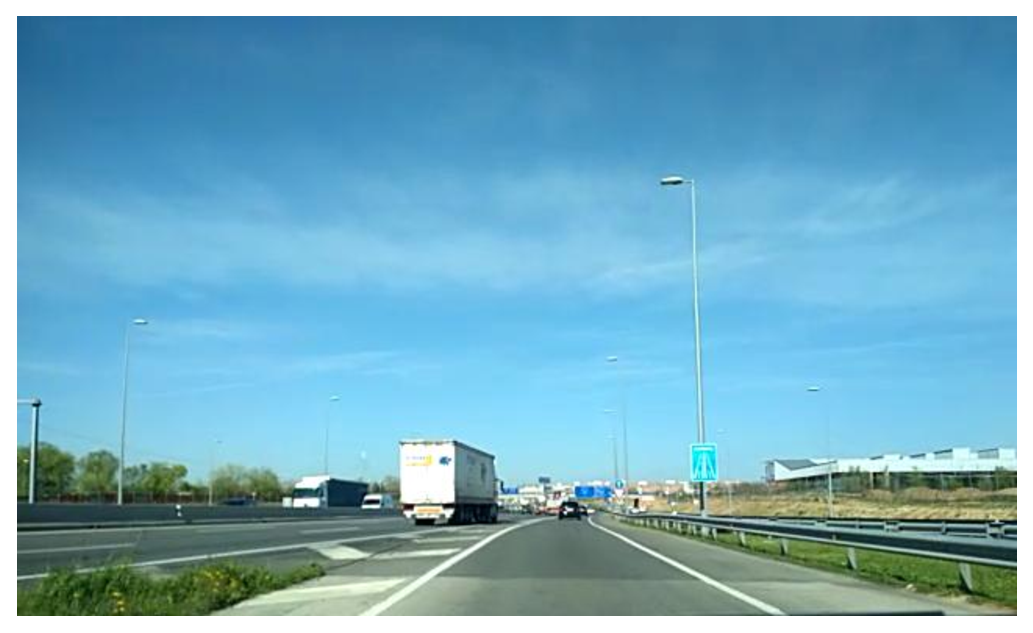
\includegraphics[width=\linewidth]{Figuras/Imagen_Original.eps}
    \caption{Imagen Original}
    \label{fig:ImgOrig}
  \end{subfigure}
    \begin{subfigure}[b]{0.45\linewidth}
    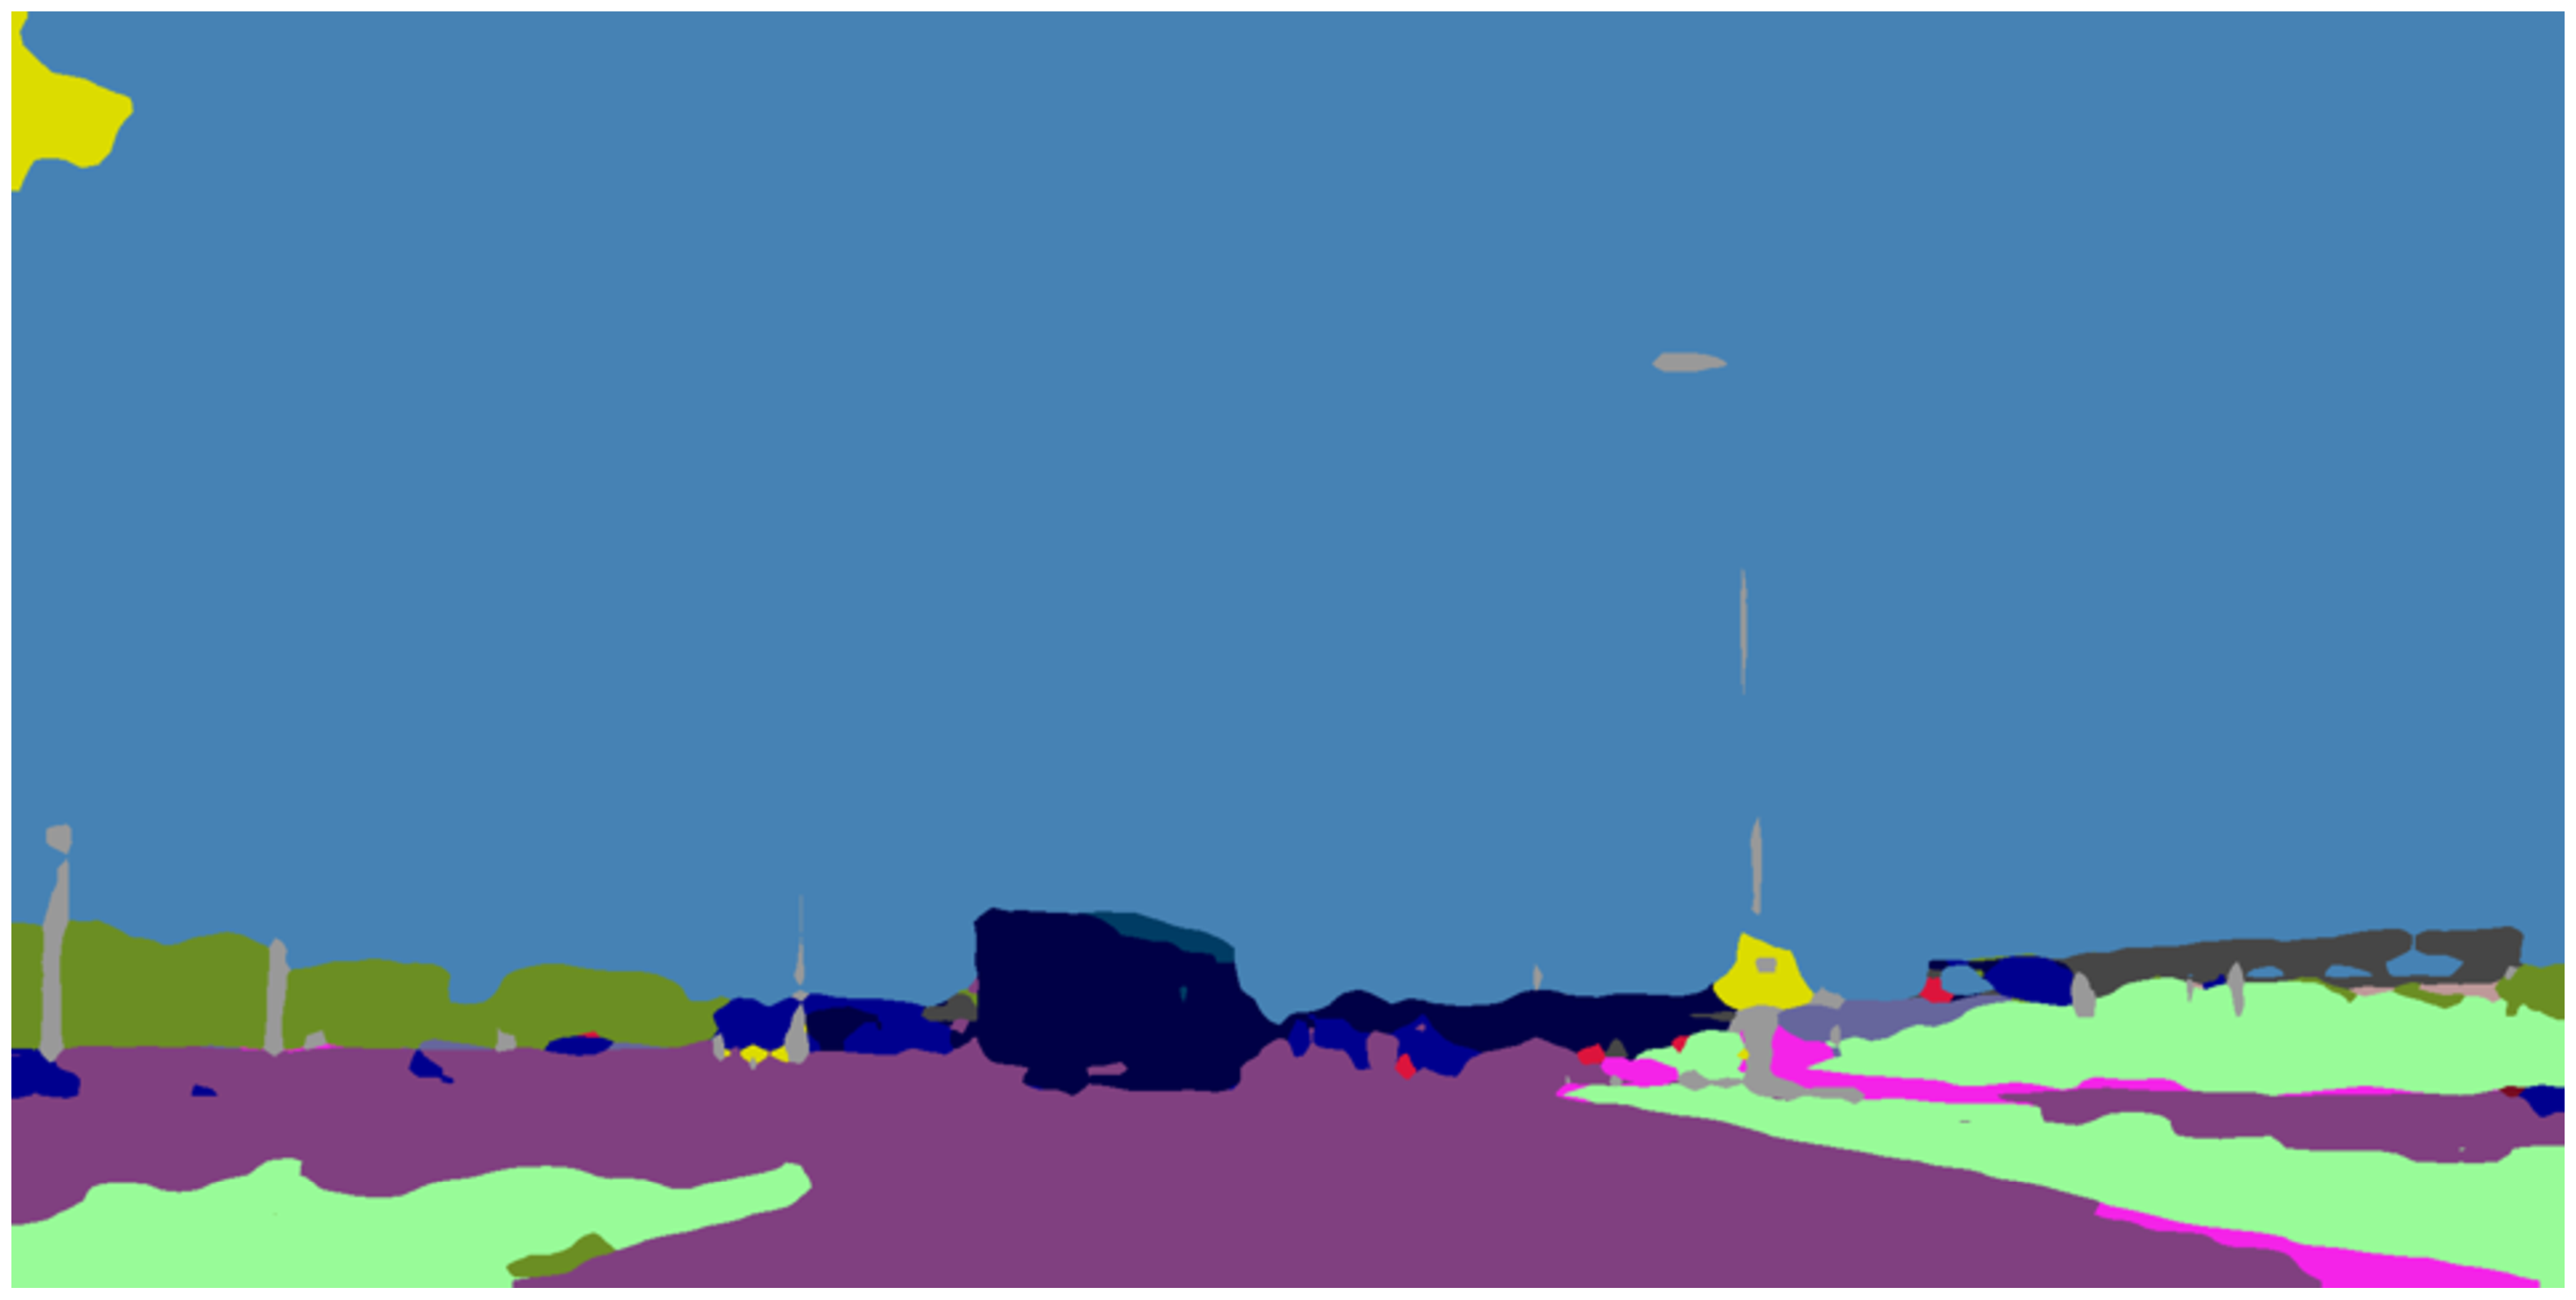
\includegraphics[width=\linewidth]{Figuras/Ejemplo_Imagen_Segmentada.eps}
    \caption{Imagen Segmentada}
    \label{fig:ImgSegm}
  \end{subfigure}
    \begin{subfigure}[b]{0.4\linewidth}
    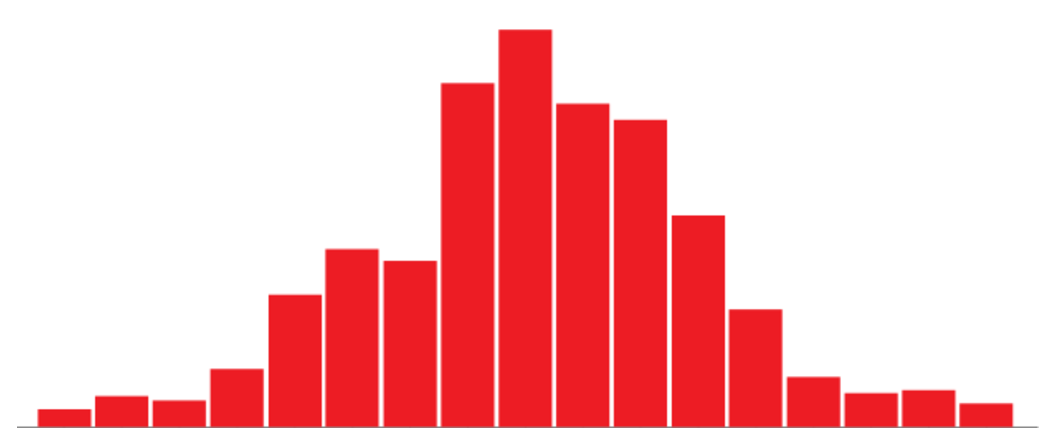
\includegraphics[width=\linewidth]{Figuras/Ejemplo_Histograma.eps}
    \caption{Ejemplo del vector de características representado como un histograma}
    \label{fig:Hist}
  \end{subfigure}
      \begin{subfigure}[b]{0.4\linewidth}
    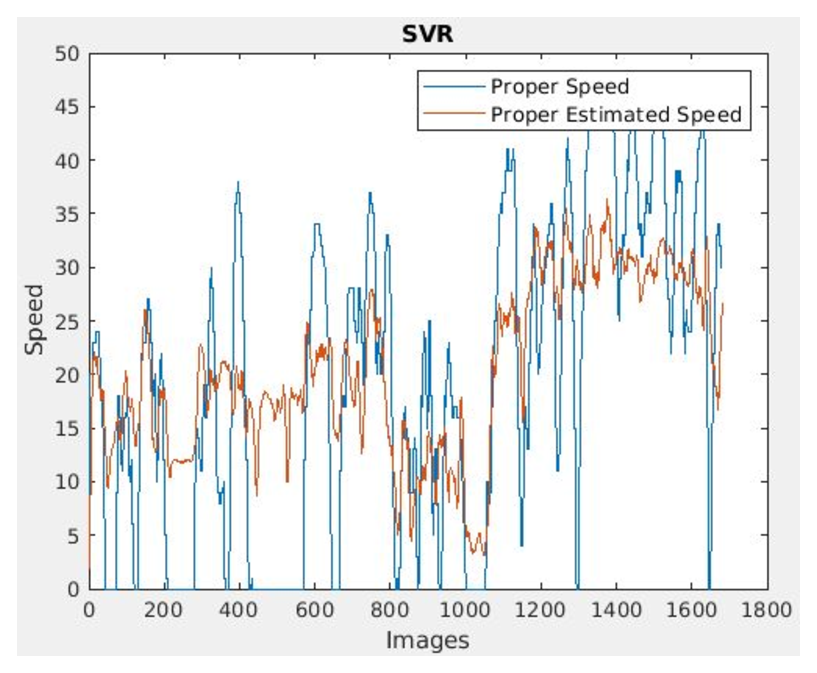
\includegraphics[width=\linewidth]{Figuras/SVR_Urban(Nivel_1).eps}
    \caption{Ejemplo de regresión final}
    \label{fig:Regre}
  \end{subfigure}
  \caption{Proceso de $ISA^{2}$}
\end{figure}

Para empezar usamos una cámara en la parte frontal del vehículo que va tomando imágenes con una cierta frecuencia (figura \ref{fig:ImgOrig}). Gracias a un sistema de \ac{SS}, conseguimos saber qué es cada cosa en cada foto, es decir; qué píxeles son los correspondientes a un vehículo, peatón, semáforo, acera, etc (figura \ref{fig:ImgSegm}). Con esa información se construye un vector de características (figura \ref{fig:Hist}) que será empleado por los módulos de inteligencia artificial para realizar una regresión o estimación de la velocidad a la que se debe circular(figura \ref{fig:Regre}).

%TODO_DONE: mejor que una imagen con solo datos de segmentación semántica, debes incluir una imagen donde se vea todo, desde la imagen original, a la segmentación semántica, y al proceso de extracción de características y la regresión final. Es para dar una idea gráfica del problema. Una vez la tengas, la metes y la comentas en el propio texto. Te dejo lo de abajo comentado para que lo cambies.

%He aquí un ejemplo de una imagen real \ref{fig:ImgOrig} y de la misma imagen procesada por el sistema de \ac{SS} \ref{fig:ImgSegm}:

%\begin{figure}[h]
%  \centering
%  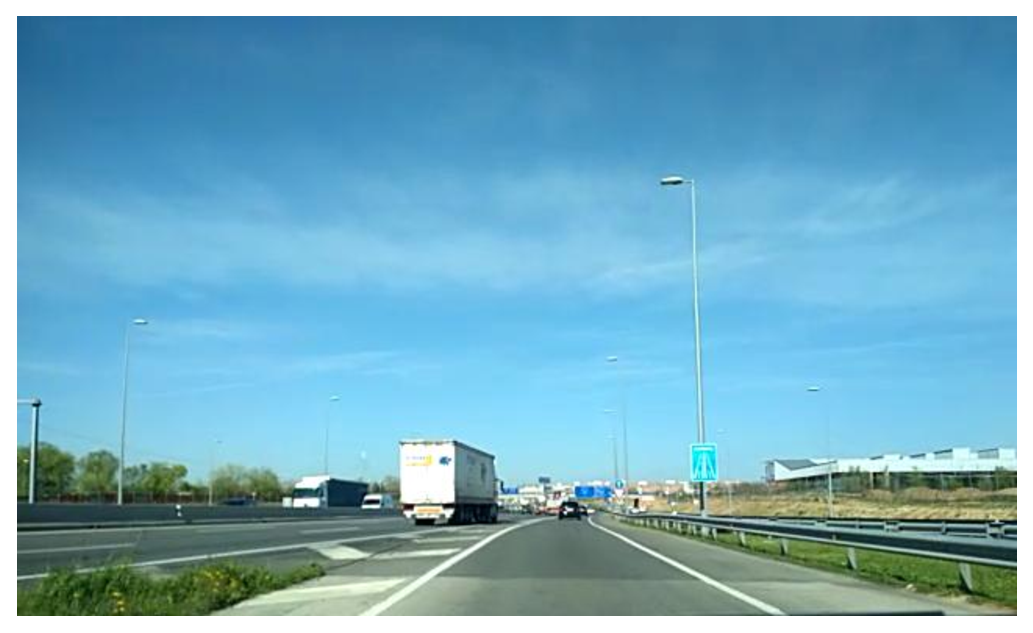
\includegraphics[width=12cm]{Figuras/Imagen_Original.eps}
%  \caption{Imagen Original}
%  \label{fig:ImgOrig}
%\end{figure}

%\begin{figure}[h]
%  \centering
%  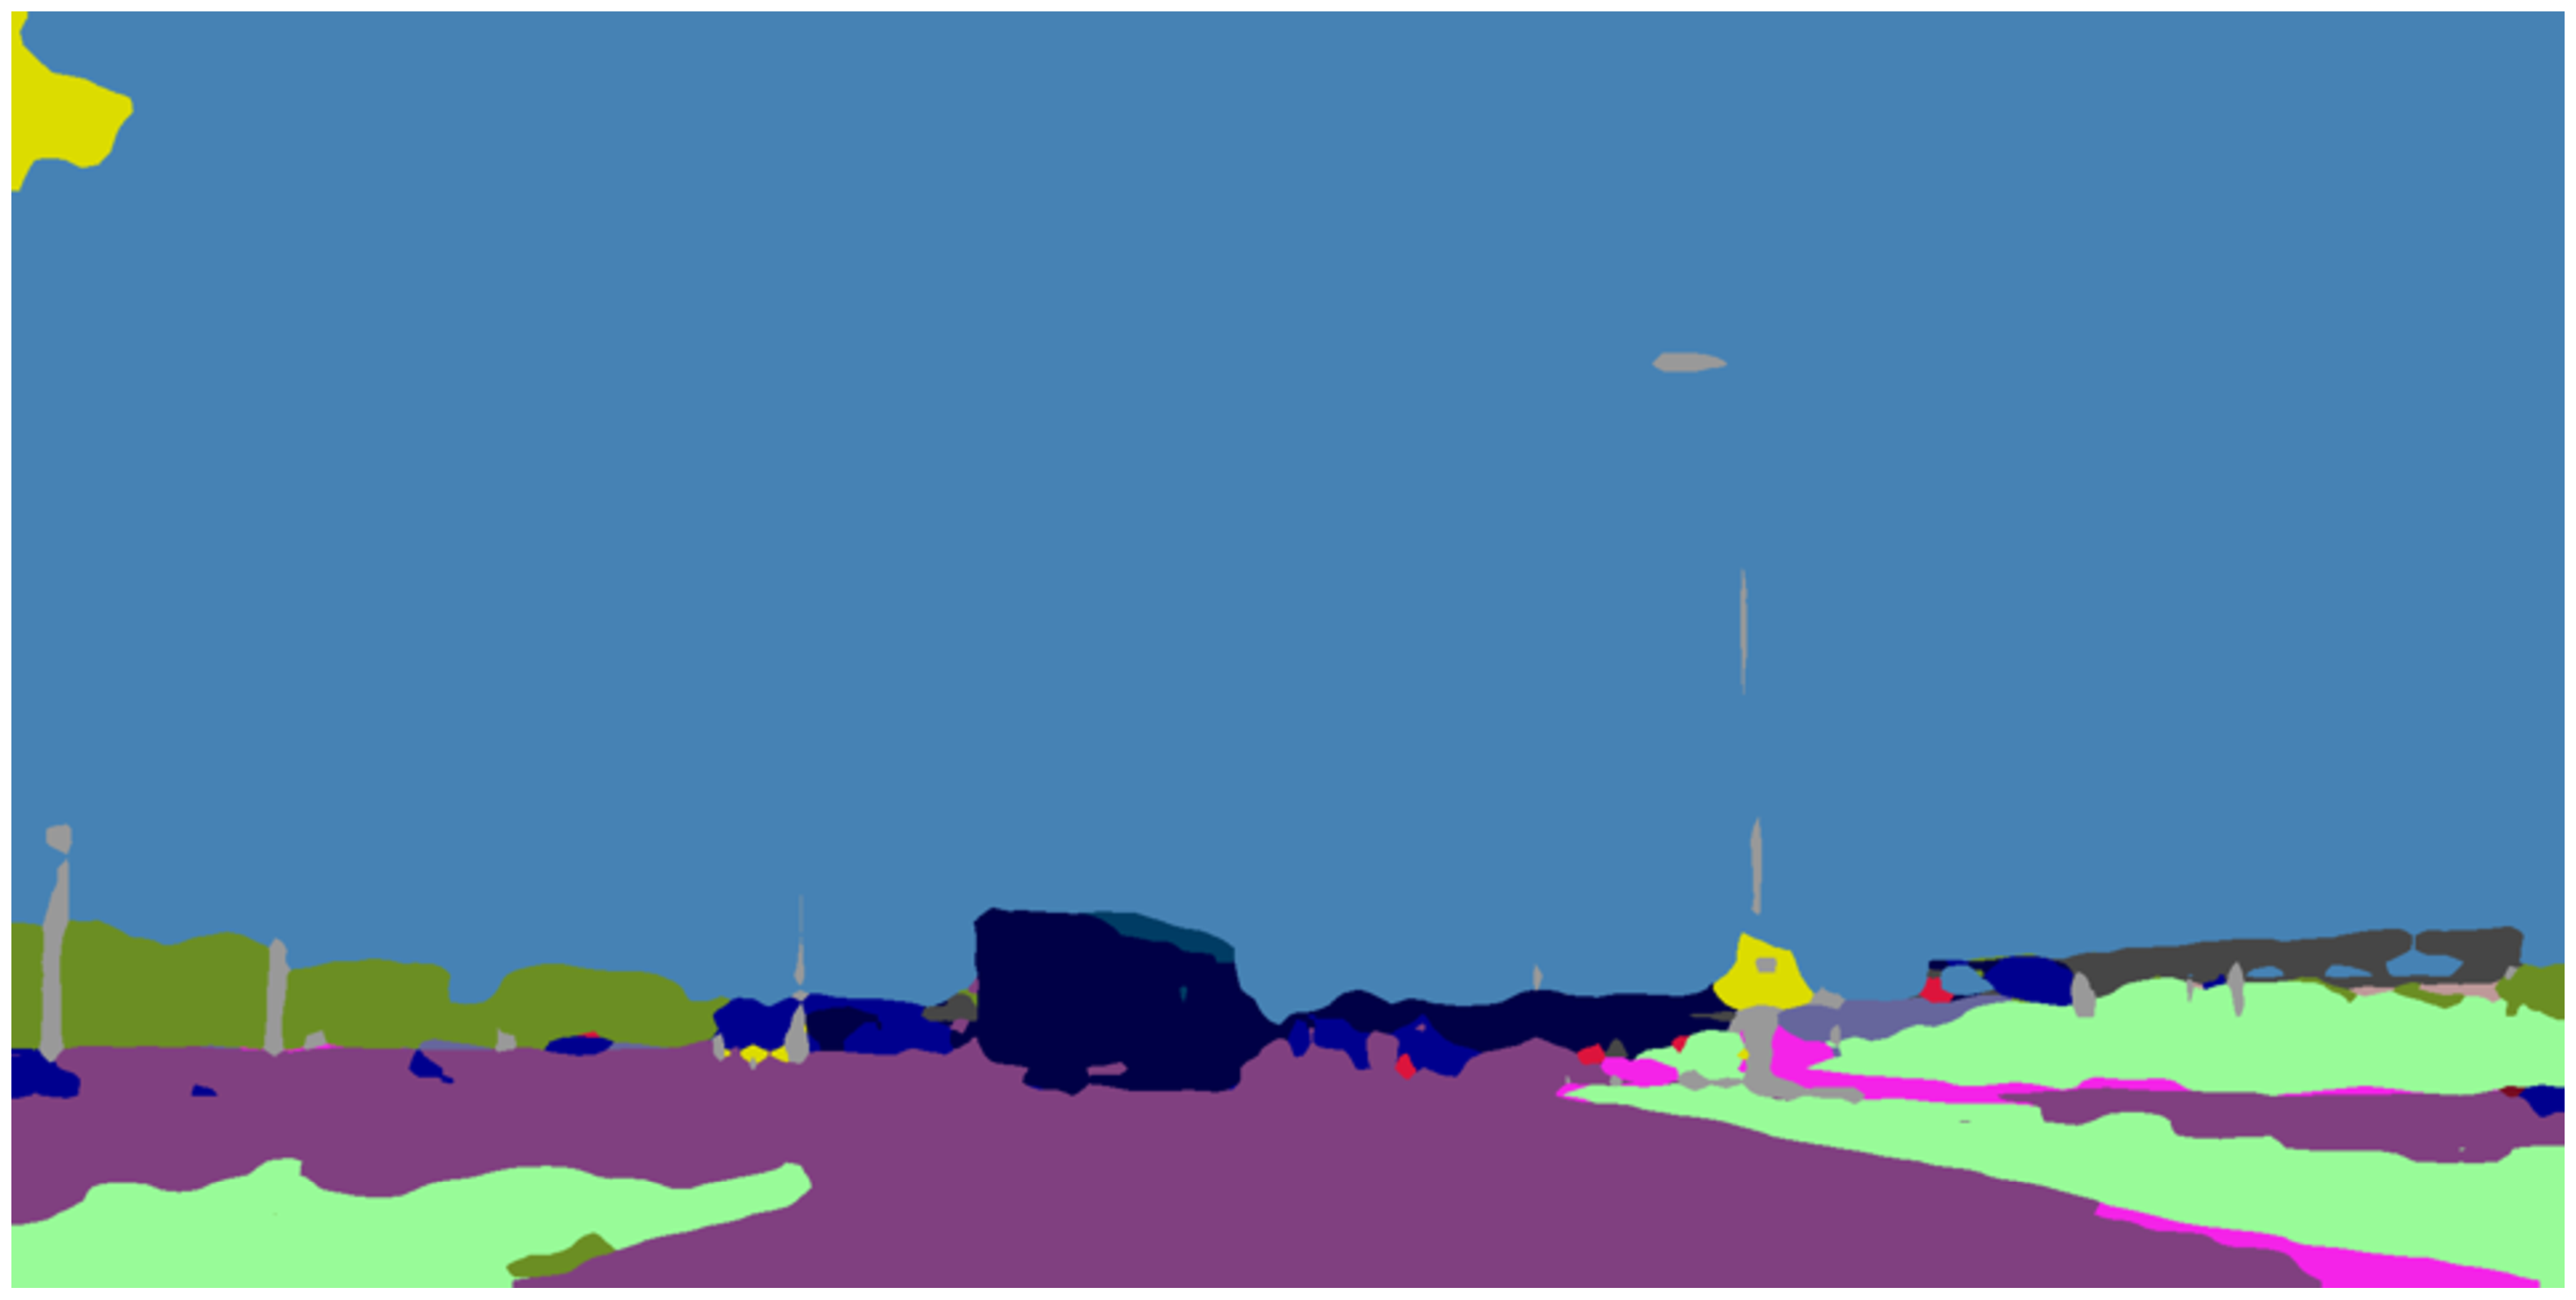
\includegraphics[width=12cm]{Figuras/Ejemplo_Imagen_Segmentada.eps}
%  \caption{Imagen Segmentada}
%    \label{fig:ImgSegm}
%\end{figure}


\section{Objetivo principal}


El objetivo principal de este proyecto es la optimización del sistema $ISA^{2}$, con respecto a la versión anterior. Para ello, partiremos de los recursos que tenemos de éste y buscaremos la mejor manera de hacerlo más práctico y eficiente.
%TODO_DONE: Sergio, lo que tenías no eran objetivos. Debes poner aquí de forma muy clara los objetivos del trabajo fin de grado.



\section{Campos de aplicación}


Este proyecto será aplicable a los sistemas de transporte inteligentes, para ayudar a mejorar la seguridad vial, facilitando una solución para controlar la velocidad a la que deben circular los vehículos. A modo de resumen, podríamos destacar las siguientes aplicaciones:
\begin{enumerate}	
	\item Implementación de soluciones de adaptación de velocidad inteligente que avisen al conductor en función de la situación real del tráfico.
	\item Implementación de sistema de detección de situaciones peligrosas en función de la velocidad.
	\item Desarrollo de nuevas ayudas a la conducción más inteligentes.
\end{enumerate}

%\section{Medios disponibles}

%Dispondremos de las siguientes herramientas:

%\begin{enumerate}
%	\item Estación de trabajo con \textbf{GPU (NVIDIA 1080 TI)} para la realización de experimentos con sistema operativo \textbf{Ubuntu}.
%	\item Acceso a la librería de \textbf{Deep Learning} llamada \textbf{PyTorch} \cite{pytorch}
%	\item Acceso a la base de datos $ISA^2$ utilizada en la primera versión \cite{isa2} a través del siguiente enlace: \url{http://agamenon.tsc.uah.es/Personales/rlopez/data/isa2/index.html}.
%\end{enumerate}

%TODO: Falta por completar la introducción con un párrafo de cierre donde explicas cómo está organizada la memoria -> "Este documento está organizado de la siguiente forma. En el capítulo 2 blablabla. El capítulo 3 incluye blablabla..."


%Incluye un capítulo cualquiera (capitulo-cualquiera.tex)
\chapter{$ISA^{2}$}
\label{ch:isa2}

Hemos hablado en la introducción sobre las soluciones \ac{ISA} a grandes rasgos y la principal novedad de $ISA^{2}$ frente a éstas. En este capítulo vamos a comenzar revisando el estado del arte (sección \ref{sec:isa2_estado_del_arte}), destacando trabajos relacionados en el ámbito de las soluciones \ac{ISA}. En la sección \ref{sec:isa2_model}, detallaremos el sistema $ISA^{2}$ sobre el que hemos trabajado en este proyecto. Finalmente, la sección \ref{sec:isa2_modelo_nuevo} incluye la descripción de los cambios que hemos implementado sobre el sistema original para hacerlo más rápido y eficaz.


\section{Trabajos relacionados}
\label{sec:isa2_estado_del_arte}

Existen soluciones comerciales para \ac{ISA} como SpeedAlert (\cite{soluciones_comerciales}) y SpeedShield basadas en tecnología \ac{GPS} proporcionando información vial (como límites de velocidad y velocidad del vehículo) y regulando la velocidad según ésta (\cite{speedshield}).

Actualmente, con la ayuda de una cámara frontal, estos sistemas son capaces de reconocer las señales de tráfico y trabajar en conjunto con una base de datos de límites de velocidad por \ac{GPS} para mantener la velocidad adecuada en cada tramo (\cite{sol_img}).

Sin embargo, ninguno de éstos puede afrontar el problema estimando la velocidad en función de la situación real del tráfico.

Lo más aproximado a nuestros intereses son una serie de trabajos que estiman la velocidad en vehículos con una secuencia de vídeos grabados por una cámara de vigilancia (\cite{isa2}, \cite{shukla}). En nuestro caso, la cámara iría en el propio vehículo distinguiendo cada parte del escenario y prediciendo la velocidad en consecuencia.

%TODO_DONE: Añadir una revisión del estado del arte en tecnología ISA. Describir primero soluciones comerciales, y cómo funcionan. Luego añadir otro párrafo de soluciones que se basen en imágenes o que sean papers que soluiones el problema. Puedes traducir y reescibir de nuevo la sección del estado del arte del paper de ISA^2.

\section{El modelo $ISA^{2}$}
\label{sec:isa2_model}

En esta sección vamos a describir cómo funciona todo el sistema $ISA^{2}$ (\cite{isa2}), centrándonos en cada parte que lo compone para que resulte más fácil su comprensión. He aquí unas figuras ilustrativas que nos servirán como punto de referencia durante todo el capítulo.


\begin{figure}[H]
  \centering
  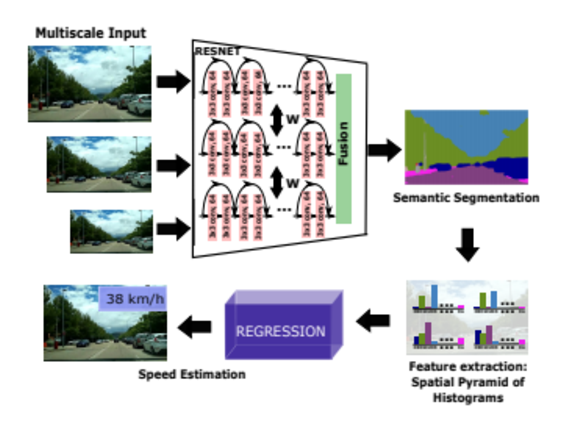
\includegraphics[width=8cm]{Figuras/Figura_Esquema_ISA2_Version_1_SegSem.eps}
  \caption{Esquema $ISA^{2}$ Antiguo.}
  \label{fig:Isa_v1}
\end{figure}

Como se puede ver al pie de la figura \ref{fig:Isa_v1} (\cite{isa2}), este fue el esquema utilizado para la primera versión de $ISA^{2}$, publicada en \cite{isa2}, cuyo funcionamiento pasamos a detallar.
%TODO_DONE: No lo hagas con item, hay que hacerlo con párrafos extensos, donde puedas resumir todo el artículo del ISA^2. Ya te anticipo que faltan bastantes detalles. El TFG no es un diario de trabajo, es un documento técnico, donde debes demostrar soltura, y reflejar los conocimientos que has aprendido.


En primera instancia el sistema recogía un set de imágenes que se correspondía con situaciones de tráfico, tanto en autovía (o autopista) como en núcleos urbanos. En concreto, la base de datos que se ofrece en \cite{isa2} consistía en dos carpetas: ``\textbf{Highway}'' y ``\textbf{Urban}'', que se correspondían con secuencias de imágenes de autovías y núcleos urbanos respectivamente. En cada una de ellas había una serie de subcarpetas en las que se almacenaban dichas secuencias; para \textbf{Highway} había dos (\textbf{H1} y \textbf{H2}) y para \textbf{Urban} tres (\textbf{U1}, \textbf{U2} y \textbf{U3}).

En ambas carpetas había \textbf{10417} imágenes en total (\textbf{4962} en Highway y \textbf{5455} en Urban).

En la siguiente figura se puede ver un ejemplo del contenido de las mismas:

\begin{figure}[H]
  \centering
  \begin{subfigure}[b]{0.45\linewidth}
    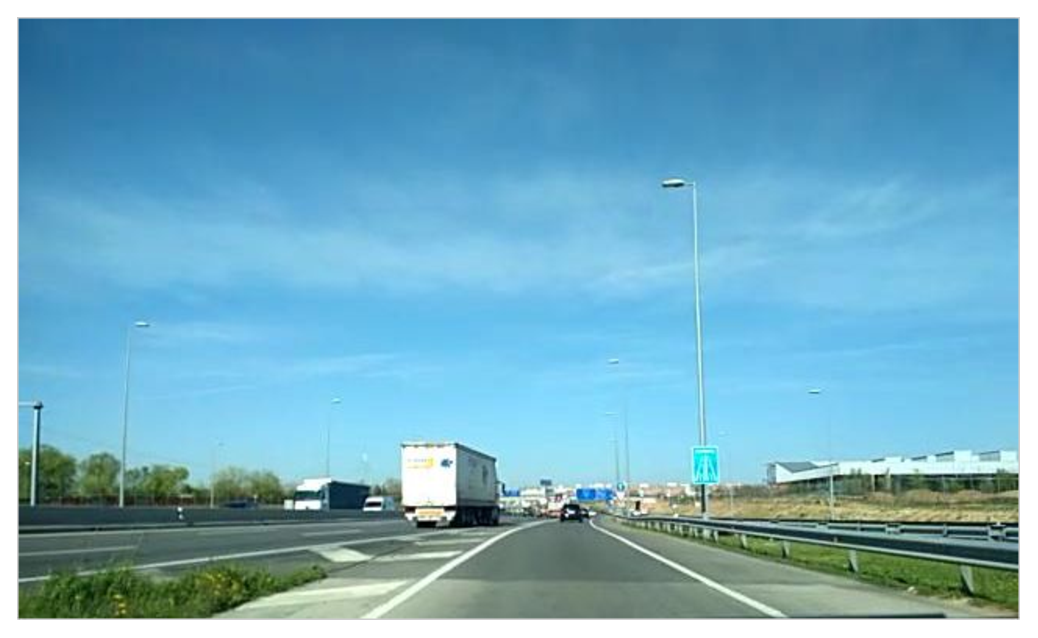
\includegraphics[width=\linewidth]{Figuras/Ejemplo_Highway.eps}
    \caption{Highway}
  \end{subfigure}
    \begin{subfigure}[b]{0.45\linewidth}
    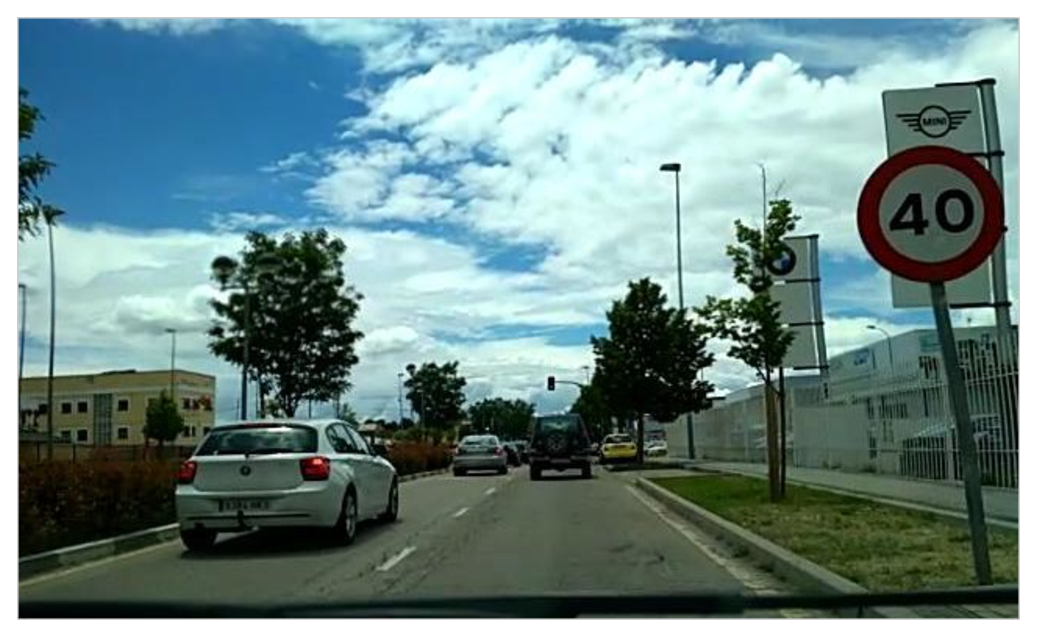
\includegraphics[width=\linewidth]{Figuras/Ejemplo_Urban.eps}
    \caption{Urban}
  \end{subfigure}
  \caption{Imágenes de $ISA^{2}$}
  \label{fig:HyU}
\end{figure}

%TODO_DONE: añade detalles de las secuencias, número de imágenes, figura con las mismas, etc.

Para cada imagen de la base de datos se dispone de la anotación de la velocidad a la que el vehículo debe de circular. Este proceso de anotación se hizo dando indicaciones a los conductores que participaron en la adquisición de las secuencias de vídeo mientras conducían. Así pues, se dispone de una base de datos con imágenes y velocidades asociadas, que se empleó para entrenar soluciones de inteligencia artificial y visión por computador, que fuesen capaces de realizar una regresión, para una imagen de entrada, de la velocidad a la que debía circular el vehículo. A continuación pasamos a describir todos los detalles de la implementación presentada en \cite{isa2}.

%TODO_DONE: Empieza a dar más detalles técnicos de todas las partes del sistema. Hay que explicar todo.
El sistema comienza realizando una \ac{SS} de la imagen de entrada. La \ac{SS} es un proceso por el cual los píxeles de una imagen son dotados de distintos valores para poder diferenciarlos en etiquetas unos de otros y así reconocer los elementos que componen dicha imagen (\cite{deeplab}). Se hace mediante el uso de modelos de inteligencia artificial configurados y entrenados para la \ac{SS}, usando en su interior herramientas de deep learning como \textbf{PyTorch} (\cite{pytorch}), de la que hablaremos más adelante. He aquí un ejemplo para mostrar el resultado del proceso:

\begin{figure}[H]
  \centering
  \begin{subfigure}[b]{0.45\linewidth}
    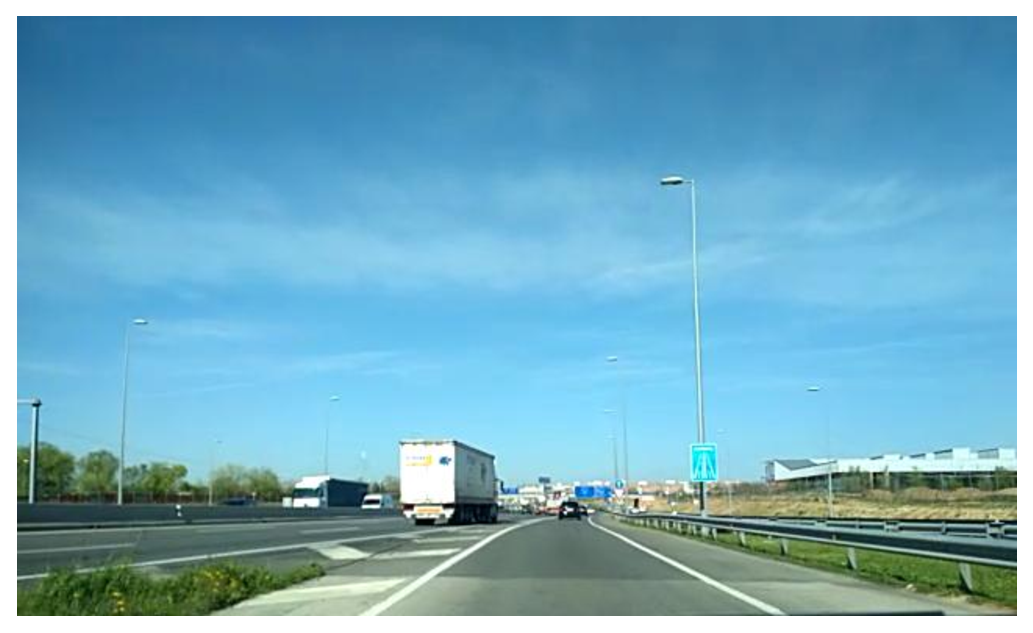
\includegraphics[width=\linewidth]{Figuras/Imagen_Original.eps}
    \caption{Imagen Original}
    \label{fig:Original}
  \end{subfigure}
    \begin{subfigure}[b]{0.5\linewidth}
    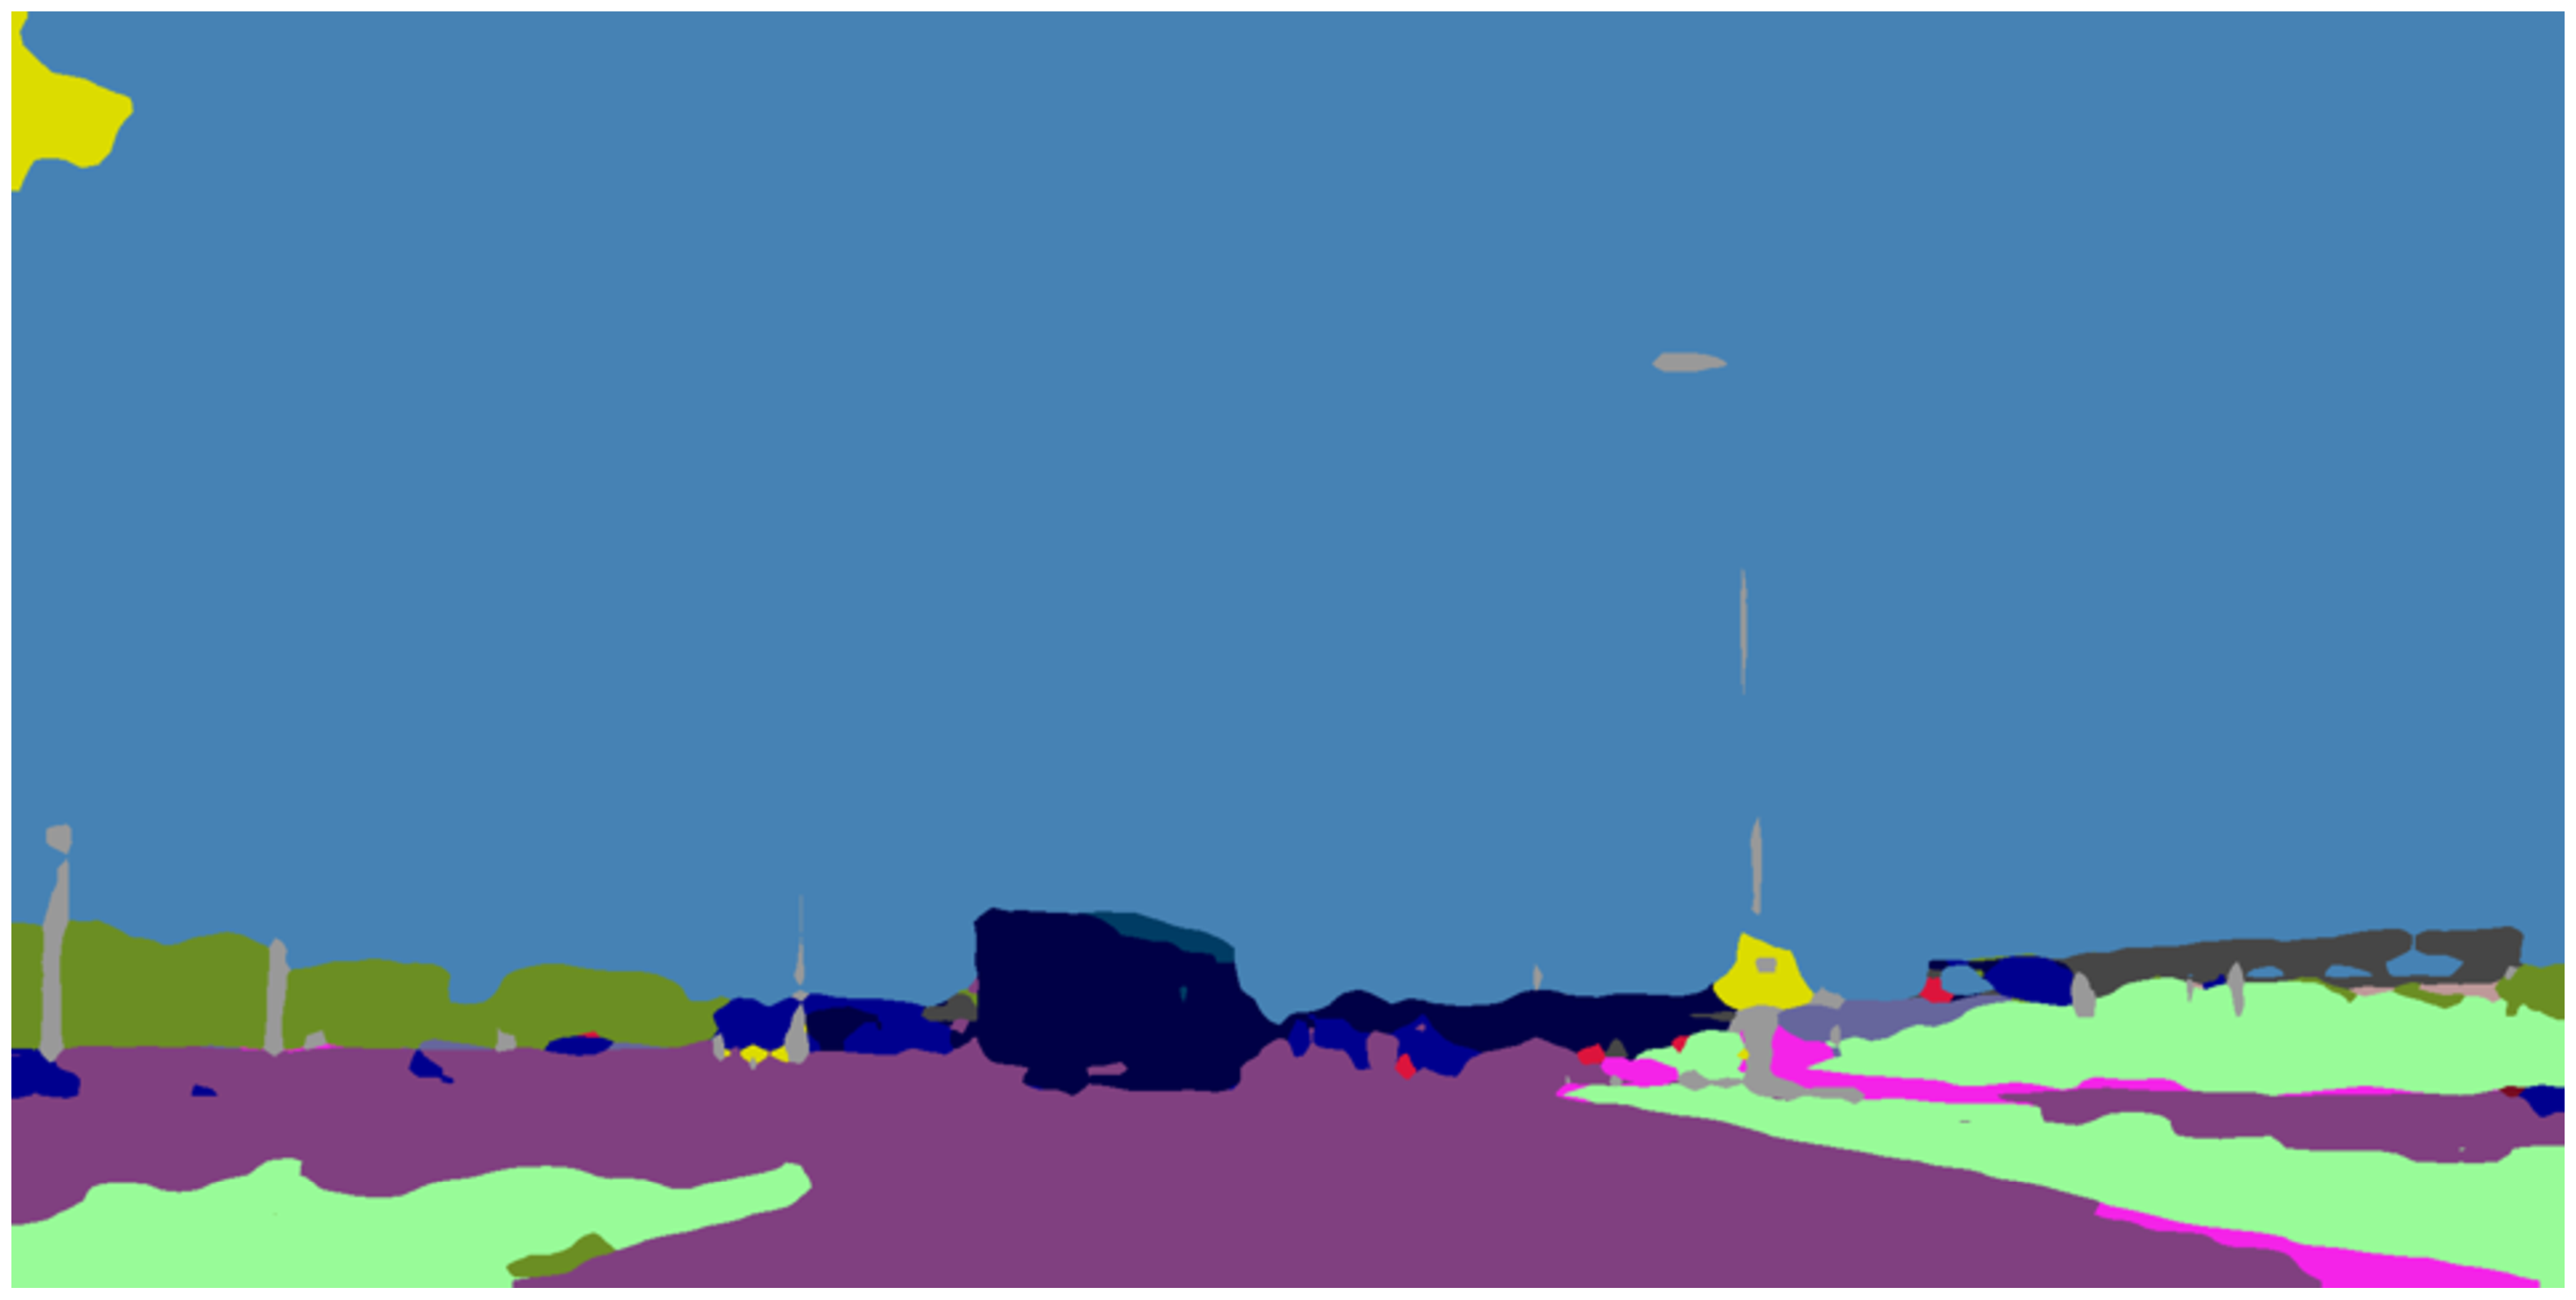
\includegraphics[width=\linewidth]{Figuras/Ejemplo_Imagen_Segmentada.eps}
    \caption{Imagen Segmentada}
    \label{fig:Segmentada}
  \end{subfigure}
  \caption{Ejemplo de \ac{SS}}
  \label{fig:SS}
\end{figure}

%TODO_DONE: añade imagen con segmentación semántica y laimagen sin segmentar, y adaptas el texto de este párrafo que de dejo comentado.
En la figura \ref{fig:SS} se puede ver la imagen de un camión, entre otros elementos, en una autovía (\ref{fig:ImgOrig}). A priori, todos los píxeles de la imagen no están categorizados y no se sabe qué partes de la imagen corresponden al camión, a la carretera, a la señal... Gracias a la segmentación semántica los píxeles de la imagen adquieren los valores de las etiquetas referentes a un \textbf{camión}, una \textbf{carretera} y una \textbf{señal de tráfico} entre otros; y son fácilmente distinguibles entre sí (\ref{fig:ImgSegm}). 

Para la \ac{SS}, el modelo en \cite{isa2} empleó la arquitectura conocida como \textbf{DeepLab} (\cite{deeplab}). \textbf{DeepLab} necesita recibir como entrada la imagen en diferentes escalas. Este modelo tenía como base una \ac{CNN}, es decir, una \textbf{Red Neuronal Convolucional} (\cite{cnn}), llamada \textbf{ResNet-101} (\cite{resnet}).

Para la primera de versión de $ISA^{2}$ en \cite{isa2}, DeepLab se entrenó con imágenes en diferentes escalas como entrada, usando factores de escalado de \textbf{0.5}, \textbf{0.75} y \textbf{1}. Más adelante se fusionaban las predicciones de la segmentación para cada escala, cogiendo la mejor respuesta dada por la red en cada una. Puesto que la base de datos de $ISA^{2}$ no tenía máscaras de segmentación (anotaciones de \ac{SS} para poder compararlas con las predicciones), DeepLab se entrenó sobre la base de datos de \textbf{Cityscapes} (\cite{cityscapes}).
%TODO_DONE: falta una breve descripción del modelo. Un párrafo es suficiente.
 

%TODO_DONE: Falta convertir estos item en párrafos como yo he hecho con el primero. Hay que explicar cada paso en detalle: los histogramas, las pirámides (qué son?, niveles?, cómo se computan?), los modelos de regresión que se probaron, etc.

Tras este proceso, mediante unos códigos de \textbf{Matlab} se recogían los datos de los píxeles ya segmentados y se organizaban en histogramas para cada imagen. Estos histogramas se organizaban según la subcarpeta de imágenes correspondiente (\textbf{H1} y \textbf{H2} para Highway y \textbf{U1}, \textbf{U2} y \textbf{U3} para Urban) para mostrar el porcentaje de píxeles referentes a una etiqueta en una determinada imagen. Basándonos en los histogramas generados, usábamos una estrategia crucial para el sistema llamada \ac{SPP} para crear un descriptor de imagen por cada histograma, los cuales usaríamos como dato de entrada para los sistemas de regresión posteriores.

Sin embargo, ¿qué es \ac{SPP} y por qué es tan importante?

\subsection{Spatial Pyramid Pooling (SPP)}

%\ac{SPP} (también conocido como ``multi-level pooling'') es una técnica usada para que cualquier imagen, en cualquier escala, pueda ser procesada correctamente por una \ac{CNN}. Consiste en la agrupación de distintas imágenes de entrada procesadas, con diferente escalado, para obtener una salida uniforme. Existen \ac{CNN}s que requieren de una escala fija en una imagen de entrada para conseguir un procesamiento óptimo, por lo que se limita la precisión de la predicción. Aplicando \ac{SPP} al final de una \ac{CNN} esta limitación desaparece.

%TODO_DONE: el párrafo anterior estaba mal, cuidado porque demuestra que no has comprendido el código del SPP. Te lo reescribo yo, pero revisa la ortografía porque voy muy rápido escribiendo.
La técnica \ac{SPP} consiste en organizar un histograma considerando la información espacial de los píxeles. En concreto, se basa en la concatenación de los histogramas, para niveles de subdivisión de la imagen. Si estamos en un nivel 1 por ejemplo, la imagen se divide en 4 secciones iguales, y se computan los histogramas por cada una de ellas, para luego ser concatenados para formar el vector final. Esto garantiza que el vector codifique de algún modo la información espacial de la imagen. A medida que aumentamos los niveles de la pirámide, aumentan de forma recurrente las divisiones y por lo tanto la granularidad del sistema. La técnica fue presentada originalmente para el problema del reconocimiento de escenas mediante visión por computador en el siguiente artículo \cite{spp_real}.
%TODO_DONE: Añade esta referencia: https://hal.inria.fr/inria-00548585/document y puedes meter como figura explicativa, una como la figura 1 de este paper.

\begin{figure}[H]
\centering
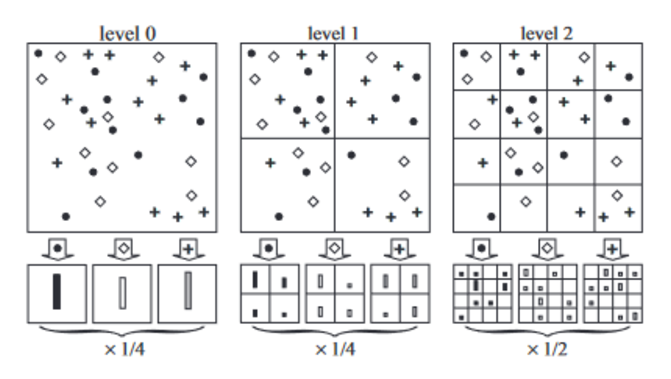
\includegraphics[width=12cm]{Figuras/SPP.eps}
\caption{Técnica \ac{SPP}}
\label{fig:spp2}
\end{figure}

Según el ejemplo de la figura \ref{fig:spp2}, podemos ver cómo se obtienen los histogramas para cada etiqueta de la imagen (representadas por círculos, diamantes y cruces). Para cada nivel de subdivisión obtenemos una serie de histogramas recogiendo los datos de las secciones de dichos niveles (como se puede ver en el nivel 1, por ejemplo). Finalmente, y tras recoger los histogramas generados se le aplica un peso a cada uno de ellos dependiendo del nivel que se use.

Una vez conseguíamos el descriptor generado en el paso anterior, éste se pasaba a diferentes sistemas de regresión (programados en MatLab): \textbf{Lineal}, \textbf{Lasso}, \textbf{Boosting Trees} y \ac{SVR}, de los cuales hablaremos más adelante. Para cada uno de ellos se añadía un cierto nivel de granularidad usando \ac{SPP} de hasta 3 niveles de agrupación para poder compararlos entre sí y saber cuál era mejor (\cite{isa2}). Para ello cogíamos los mejores resultados de cada sistema entre todos los niveles usados, y los usábamos como referencia del modelo $ISA^{2}$.

%TODO_DONE: toda esta subsección hay que moverla al capítulo de resultados, donde explicas la métrica

\section{Propuesta de modelo $ISA^{2}$ mejorado}
\label{sec:isa2_modelo_nuevo}
El trabajo fundamental de este TFG ha consistido en mejorar el sistema tradicional $ISA^{2}$. Nuestro objetivo con este TFG es el de conseguir un sistema $ISA^{2}$ que pueda funcionar en tiempo real, y que consuma pocos recursos de \ac{GPU}, para poder ser embebido en una plataforma de procesado dentro de un vehículo inteligente. La solución descrita en \cite{isa2} no cumplía ninguno de estos requisitos, principalmente por el sistema DeepLab para segmentación semántica que llevaba integrada. DeepLab es un modelo que da excelentes prestaciones en cuanto a segmentación semántica se refiere, pero no funciona en tiempo real, y además necesita una tarjeta de procesado con mucha memoria de \ac{GPU} y muy alto consumo.

Los modelos en tiempo real tienen, como principal objetivo, cumplir con los resultados de un modelo basado en \ac{DCNN} como DeepLab, ya que éstos son los que mejores prestaciones suelen dar debido a los recursos computacionales tan potentes que usan, sin los inconvenientes que ellos mismos traen consigo. Modelos como ERFNet (\cite{erfnet}) o ICNet (\cite{icnet}) lo consiguen usando arquitecturas más ligeras en comparación (aunque no sean las adecuadas para el reconocimiento de imágenes a gran escala).

Uno de los inconvenientes más importantes de los modelos en tiempo real es el campo de visión (\cite{swiftnet}). El campo de visión es realmente grande cuando se trabaja con modelos como DeepLab porque su arquitectura puede soportar tales cantidades de información mientras que en los modelos en tiempo real, éste se reduce. Es por ello que actualmente se tratan con técnicas como \textbf{pirámides de resolución} (\textit{resolution pyramids}) o \textbf{conexiones laterales} (\textit{lateral connections}) para compensarlo (\cite{res_pyr}, \cite{lat_con}).

Por otro lado, la principal ventaja (y la más evidente) de estos modelos es el bajo consumo de \ac{GPU} en comparación, además del uso de arquitecturas mucho más ligeras que en la otra clase de modelos. Esto hace posible que el procesado de imágenes sea más rápido y, por lo tanto, la toma de decisiones también.

Como ya hemos dicho lo ideal sería encontrar un modelo en tiempo real que pueda detectar los objetos de las imágenes con una precisión exquisita, y con un bajo consumo de la \ac{GPU}, y poco a poco se está consiguiendo.
%TODO_DONE: Sigue motivanto tú el trabajo, saca información del artículo siftwnet. en la intro se ve que hay familias de modelos que funcionan en real-time, ventajas, inconvenientes.


En resumen, para conseguir un modelo $ISA^{2}$ más rápido y eficaz, hemos decidido cambiar el sistema de segmentación semántica Deeplab por el conocido como \textbf{Swiftnet} (\cite{swiftnet}). La idea puede verse reflejada en la Figura \ref{fig:Isa_v2}.

\begin{figure}[H]
  \centering
  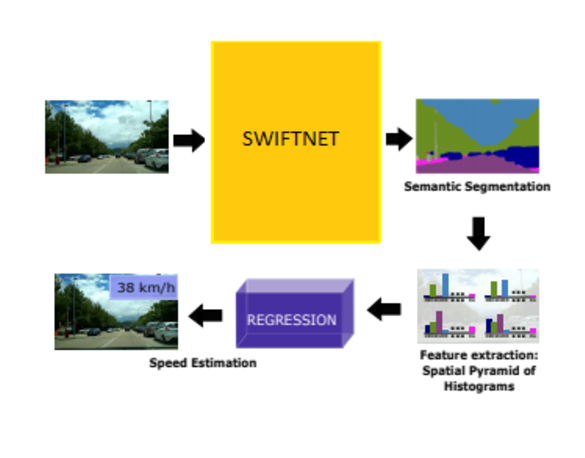
\includegraphics[width=8cm]{Figuras/Figura_Esquema_ISA2_Version_2.eps}
  \caption{Esquema $ISA^{2}$ Actual}
    \label{fig:Isa_v2}
\end{figure}


Como se puede comprobar, el esquema de la figura \ref{fig:Isa_v2} sigue el mismo camino que el de la primera versión, salvo por unas modificaciones al principio que pasamos a explicar a continuación:

\begin{enumerate}

\item Las imágenes de entrada al modelo de \ac{SS} no llegan en diferentes escalas como se podría intuir. La razón de por qué es así es Swiftnet: el modelo admite tanto imágenes en diferentes escalas como imágenes con una única escala. Sin embargo, para este proyecto hemos optado por la recomendación de los autores (\cite{github_swiftnet}) y hemos decidido hacerlo con una única escala. De esta manera hemos obtenido los resultados esperados con la base de datos de \textbf{Cityscapes} (\cite{cityscapes}) que ellos mismos utilizaron (\cite{swiftnet}).

\item La segunda, y última, modificación es la más obvia: la sustitución del modelo de DeepLab por el modelo de Swiftnet (\cite{swiftnet}). A diferencia del primero, Swiftnet es un modelo que opera en tiempo real (\textbf{Real-Time}) de tal modo que cuando procesa una imagen lo hace en el momento, a una tasa de 39.9 \ac{FPS} (para la base de datos de Cityscapes, que es con la que extrajo este dato).%TODO_DONE: añade la velocidad a la que funciona en frames por segundo, seguro que viene en el paper original de siftnet.

\end{enumerate}


En el siguiente capítulo hablaremos acerca de la implementación de Swiftnet y de cómo es mejor para los campos de aplicación, especificados anteriormente, con respecto a DeepLab.


\chapter{Implementación}


A la hora de implementar esta nueva arquitectura debemos considerar que, para ejecutarla, hay que crear un entorno, un escenario, real sobre el que hacerlo. O, en su defecto, crear un entorno que simule esas condiciones para trabajar con ella.

Es por ello que antes de trabajar con el modelo de ``Swiftnet'' \cite{swiftnet} tenemos que sentar las bases sobre las que se pueda ejecutar. Así comienza la creación de un entorno Conda.

\section{Conda}

Conda \cite{conda} es un sistema de gestión de entornos con el que creamos el escenario sobre el que vamos a correr ``Swiftnet'' \cite{swiftnet}. Conda permite crear el escenario instalando y gestionando paquetes de uso público ubicados en diferentes ``canales'' del sistema. Simplemente hay que seguir las instrucciones que dan para descargarlos e instalarlos, y poder añadirlos así al escenario sobre el que se esté trabajando.

\begin{figure}[H]
  \centering
  
\includegraphics[width=8cm]{Figuras/Conda.eps}
  \caption{Conda}
\end{figure}

Antes de crear ningún entorno, primero hay que instalar Conda en la máquina que va a procesar el proyecto. Para ello descargamos Miniconda (un instalador de Conda) para Python 2.7 \cite{miniconda_install}. Una vez descargado ya podemos crear entornos Conda.


Para crear el entorno Conda sobre el que trabajar basta con abrir un terminal del sistema operativo y escribir el siguiente comando:

\begin{center}
\textit{conda  create  --name  swiftnet  python=3.7}
\end{center}

En este caso estamos creando un entorno Conda llamado ``swiftnet'' con la versión de Python 3.7 (la necesaria para el modelo de ``Swiftnet'', aunque se admiten versiones superiores  \cite{github_swiftnet}).


Ya tenemos creado el entorno, ahora hace falta añadirle los paquetes necesarios que requiere ``Swiftnet'', indicados en el archivo ``requirements.txt'' \cite{github_swiftnet}. Para instalarlos simplemente seguimos las indicaciones del modelo y usamos este comando:

\begin{center}
\textit{pip install -r requirements.txt}
\end{center}

``Pip'' es otro gestor de paquetes que, junto a Conda, es muy útil a la hora de instalar aquellos paquetes que Conda no posee en sus ``canales'' \cite{pip}.

Con el anterior comando, se instalan una serie de paquetes necesarios para la ejecución del modelo, entre ellos PyTorch \cite{pytorch}, del cual hablaremos más adelante; pero no todos (en nuestro caso). Para que el modelo funcione correctamente hay que instalar los restantes con este comando \cite{conda_sheet}:

\begin{center}
\textit{conda install nombre\_del\_paquete -c nombre\_del\_canal\_en\_el\_que\_se\_encuentra\_el\_paquete}
\end{center}

A continuación enumeramos los paquetes que quedan para poder ejecutar ``Swiftnet'':

\begin{enumerate}
\item opencv \cite{opencv}
\item pytorch torchaudio=0.4.0 cudatoolkit=10.0 \cite{pytorch}
\end{enumerate}

Cabe destacar que ponemos dichos paquetes con estas versiones porque las especificaciones de nuestra máquina lo requerían. Si se quiere reproducir el resultado de este proyecto, puede que no sean las mismas versiones de estos paquetes los que haya que instalar, dependerá de la máquina sobre la que se trabaje.

Una vez instalados dichos paquetes, se sigue el procedimiento marcado por el modelo (se descargan la base de datos de Cityscapes \cite{cityscapes} y una serie de modelos preentrenados para la misma en la carpeta ``weights'' \cite{github_swiftnet}) y se ejecuta desde el directorio en el que éste se encuentra:

\begin{center}
\textit{python eval.py configs\textbackslash{rn18\_single\_scale.py}}
\end{center}

Tras ello, y en nuestro caso particular, se llegarán a dos errores:

\begin{enumerate}
\item No se encuentra el módulo ``lib.cylib''
\item No se encuentra la versión ``GLIBCXX\_3.4.26'' de ``libstdc++'' que se encuentra en el sistema operativo
\end{enumerate}

Pasamos a explicarlos:

\subsection{Error de ``lib.cylib''}

Este error se da porque aún no se ha creado módulo de ``cython'' \cite{cython} necesario para evaluar las métricas del modelo. Se consigue ejecutando el código del archivo ``build.sh'' del modelo en la carpeta ``lib\textbackslash{}'' de éste.

Sin embargo, antes de ejecutarlo conviene modificarlo de la siguiente manera:

\begin{figure}[H]
  \centering
  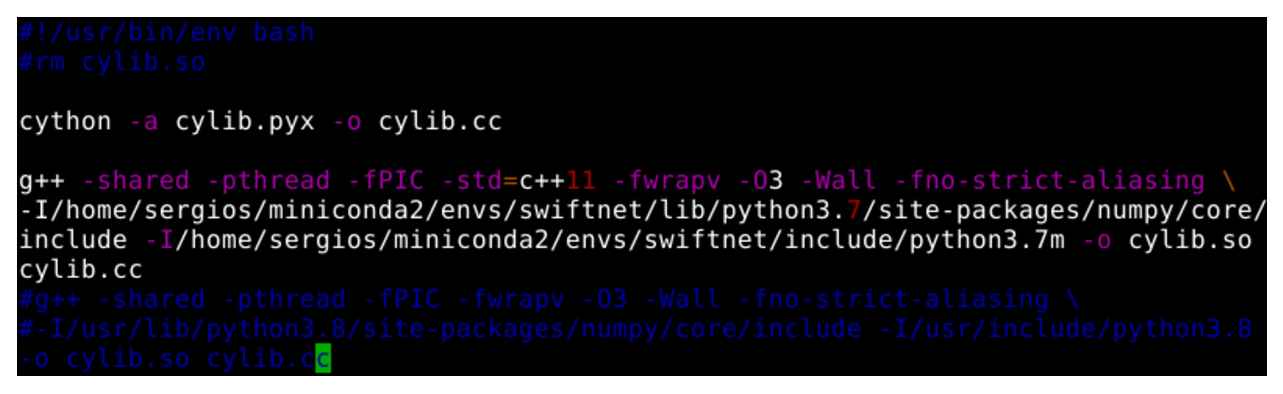
\includegraphics[width=12cm]{Figuras/cylib.eps}
  \caption{Archivo ``build.sh''}
  \label{fig:cylib}
\end{figure}

Tras hacerlo, lo ejecutamos con el siguiente comando:

\begin{center}
\textit{.\textbackslash{build.sh}}
\end{center}

Si nos sale algún error porque falta algún paquete por instalar, volvemos al comando que utilizamos para instalar paquetes por Conda y los instalamos de forma sencilla.

Como se puede observar en la figura \ref{fig:cylib}, el archivo está en ``Shell Script'' \cite{shell} y a través de éste se crean los archivos ``cylib.so'', ``cylib.cc'' y ``cylib.html''.

Cabe destacar otra observación muy importante en la figura: Hay que modificar las líneas en las que se hace referencia al sistema de archivos propio de la máquina sobre la que se trabaja.

En nuestro caso, tenemos la siguiente ruta seguida de los directorios que se han creado al haber instalado los paquetes previos a la ejecución del modelo:

\begin{center}
\textit{\textbackslash{home}\textbackslash{sergios}\textbackslash{miniconda2}\textbackslash{envs}\textbackslash{swiftnet}}
\end{center}

Es muy importante cambiar esa ruta por la de la máquina sobre la que se trabaje, si no, no puede funcionar; de modo que cuando se instale Conda y se cree el entorno sobre el que se quiere trabajar, hay que tener muy en cuenta dónde se instala para modificarla.

Por otro lado, el resto de la ruta no se cambia, ya que son paquetes comunes a cualquier usuario que intente ejecutar ``Swiftnet'' \cite{swiftnet}.

Por último, puntualizar que la última parte comentada del archivo, que es muy similar a la que hemos modificado hace un momento, sirve para lo mismo pero utilizando Python 3.8. Si se quisiese utilizar este modelo con esa versión de Python habría que descomentarla y comentar la referente a Python 3.7. Lo demás se mantendría como está.

\subsection{Error de ``GLIBCXX''}

Para empezar, ``libstdc++'' \cite{glibcxx} es la implementación de la librería estándar del lenguaje C++ de programación.

Esto quiere decir que para cualquier programa en C++ que use hilos o archivos, por ejemplo, usará esta librería para implementar lo pertinente a estas cosas en las librerías de C++.

Por otro lado tenemos la \ac{ABI} \cite{glibcxx}, la cual sirve para que, por ejemplo, un programa compilado en ``libstdc++'' en 2013 funcione de la misma manera para una nueva versión de ``libstdc++'' en 2021. Cuando se actualiza esa librería y se quiere compilar un programa de una versión anterior, se mantiene la ABI de dicha versión para compilar ese programa.

Sin embargo, cuando se actualiza ``libstdc++'' y se mantiene su ABI, cada función o símbolo de dicha librería obtiene una nueva versión, a la que se le llama mediante un ``linker''.

El ``linker'' enlaza la llamada a una función de la librería con su última versión \cite{glibcxx}.

Para nuestro caso, no encuentra la versión ``GLIBCXX\_3.4.26'' de ``libstdc++'' debido a que el ``linker'' no tiene permisos para acceder a la librería del sistema operativo. Por lo que, cada vez que ejecutemos el modelo, aunque lo intente, no podrá encontrar dicha librería.

Sin embargo, he aquí una razón de uso de los entornos Conda: Cuando se crea un entorno Conda nuevo, éste también adquiere esta librería al venir incluida en uno de los paquetes de instalación predeterminados para la creación del entorno. De este modo obtenemos la versión que requiere ``Swiftnet'' para su ejecución.

Aún así sigue existiendo un problema: el ``linker'' sigue buscando la versión requerida por ``Swiftnet'' en el mismo lugar, de modo que cada vez que se llame a esa librería el ``linker'' seguirá buscando donde siempre y seguiremos igual. La solución reside en hacerle saber al ``linker'' dónde buscar esta nueva versión, y para ello usaremos este comando en la terminal:

\begin{center}
\textit{export LD\_LIBRARY\_PATH=\$LD\_LIBRARY\_PATH:\$HOME\textbackslash{miniconda2}\textbackslash{lib}\textbackslash{}}
\end{center}

No obstante, esta solución sirve siempre y cuando no se cierre la terminal. En el momento en el que se cierre hay que volver a abrir otra y volver a utilizarlo.

Al usarla, conseguimos nuestro objetivo y podemos seguir avanzando en la ejecución del modelo.

\section{PyTorch}

Anteriormente lo hemos mencionado, y a diferencia de otros paquetes de instalación, éste conviene explicarlo, pues es en lo que se basa ``Swiftnet'' para hacer la \ac{SS}.

\begin{figure}[H]
  \centering
  
\includegraphics[width=8cm]{Figuras/PyTorch.eps}
  \caption{PyTorch}
\end{figure}

PyTorch \cite{pytorch} es un framework de Python de ``deep learning'' que permite su utilización en aplicaciones que implementan visión por computador o IA. Está basado en la librería ``Torch'', de ahí que los paquetes que se requieren instalar por Conda tengan el mismo nombre y derivados.

PyTorch trabaja, entre otras cosas, con ``tensores'', que sirven para operar con arrays de n-dimensiones. Este tipo de variables se usan durante todo el modelo de ``Swiftnet'' ya que son las que obtendrán, por ejemplo, la lectura de datos de las imágenes, la información de las clases de las etiquetas (persona, vehículo...).

En esencia, PyTorch posibilita la existencia del modelo de ``Swiftnet''. Si no se utilizase, podríamos utilizar otros como Tensorflow \cite{tensorflow} o Caffe \cite{caffe}, sin embargo, cada uno de estos frameworks está enfocado hacia diferentes aspectos y habría que analizar cuál de ellos podría ser el adecuado para el modelo. 

PyTorch se puede instalar tanto para máquinas con tarjeta gráfica como sin ella, dependiendo de cómo se quiera ejecutar. Generalmente, se suele instalar en máquinas con tarjeta gráfica y por ello se instala, además de los paquetes de ``Torch'', el paquete ``cudatoolkit''. Este paquete interactúa con CUDA \cite {cuda}.

\subsection{CUDA}

CUDA \cite{cuda} es una plataforma desarrollada por NVIDIA para poder trabajar, a nivel de cómputo, con las \ac{GPU}.

Como ya hemos dicho, el paquete ``cudatoolkit'' es necesario para trabajar con PyTorch en máquinas con tarjeta gráfica (\ac{GPU}). Sin embargo, es posible instalarlo y poder ejecutar PyTorch sin la \ac{GPU}, es decir, a través de la \ac{CPU}.

Basta con hacerle saber a PyTorch sobre qué ejecutarlo con la siguiente instrucción:

\begin{center}
\textit{torch.device(`cpu/gpu')}
\end{center}

Escribiendo dicha instrucción en el código que se quiera ejecutar especificando una de las dos opciones que se dan (\ac{CPU} o \ac{GPU}), podemos obligar a PyTorch a que trabaje con una u otra.


En cuanto a términos de rendimiento, es recomendable ,si es posible, que PyTorch trabaje con \ac{GPU} puesto que al hacerlo de la otra forma, la carga de procesos que tendría que soportar la \ac{CPU} sería elevada y conllevaría a que tardase demasiado la ejecución del modelo. Con \ac{GPU}, sin embargo, sería más veloz y podríamos trabajar con mayor soltura al no tener largos tiempos de espera durante la ejecución del modelo.


\section{Swiftnet}

Ya hemos explicado las bases sobre las que se sustenta ``Swiftnet'' (PyTorch y CUDA) y sobre dónde ejecutarlo (entorno Conda), además de explicar y solucionar los errores que pueden ocurrir durante el proceso. A continuación pasamos a explicar el propio modelo y cómo ejecutarlo paso a paso.

\subsection{Cityscapes}

Para la ejecución del modelo tomaremos como referencia la base de datos de Cityscapes \cite{cityscapes}, como viene indicado en la guía de éste \cite{github_swiftnet}, para poder comparar los resultados con los del paper de ``Swiftnet'' \cite{swiftnet}.

Antes de continuar, es recomendable cambiar el nombre de las bases de datos que se han descargado de Cityscapes por nombres más sencillos por comodidad. En nuestro caso, llamamos ``labels'' a la carpeta que contiene las etiquetas de las imágenes (241 MB) y ``rgb'' a la carpeta que contiene las imágenes (11 GB).

Cuando esté descargada la base de datos, vamos a la carpeta referente a las etiquetas (``labels''). Una vez dentro, tenemos que, o bien borrar todos los archivos ``instanceIds'' y ``color'', o bien moverlos en otra carpeta. Esto es porque durante la ejecución del modelo, éste podría confundirse de archivos y coger los que queremos borrar (o mover), y nos interesa que utilice sólo los llamados ``labelIds''.

También aparecen unos archivos con la extensión ``.json'' que es conveniente dejarlos tal y como están.

\subsection{Pycharm}

Para ejecutar ``Swiftnet'' nos hemos ayudado de un \ac{IDE} llamado ``Pycharm'' \cite{pycharm}.

``Pycharm'' nos sirve para poder comprobar la ejecución del modelo paso a paso. De otra manera, si lo hiciéramos desde la terminal, resultaría mucho más difícil saber cómo procesa las imágenes. Se puede descargar de manera muy sencilla.

\subsection{Proceso de Swiftnet}

Una vez tenemos ``Pycharm'' podemos pasar a ejecutar ``Swiftnet'', el cual funciona de la siguiente manera:

\begin{enumerate}
\item En primera instancia, ``Swiftnet'' carga las especificaciones del archivo de configuración ``rn18\_single\_scale.py'' que pasaremos a modificar a continuación.
\item Más adelante, carga la información de las clases de las etiquetas (persona, carretera, vehículo...).
\item A continuación, carga el modelo de \ac{SS} que se va a utilizar con CUDA \cite{cuda}.
\item Por último, evalúa el modelo cargado usando las imágenes del dataset de Cityscapes, la información de las clases, etc... Para evaluarlo sigue los siguientes pasos:

\begin{itemize}
\item Crea una pila para guardar las predicciones que se van a hacer de las imágenes de Cityscapes. Con ``predicciones'' nos referimos a ``imágenes segmentadas por el modelo''.
\item En la pila creada, se colorizarán las etiquetas de las predicciones y se formarán éstas. En esencia, la pila será la encargada de realizar estas funciones además de guardar los resultados en el directorio adecuado
\item Una vez se crea la pila, se crean lotes de imágenes que van a pasar por el modelo para que éste los vaya segmentando, es decir, que vaya etiquetando las imágenes del lote según las clases que detecte.
\item Una vez todo finaliza, se calcula el porcentaje de acierto que ha tenido el modelo con las imágenes reales. De ahí se extraen los datos que aparecen en el paper de ``Swiftnet''.
\end{itemize}   
\end{enumerate}

Sin embargo, si lo ejecutamos siguiendo el comando que nos dice el procedimiento del modelo no funcionará.

Esto es porque antes de ejecutarlo debemos modificar el archivo ``rn18\_single\_scale.py'' de la carpeta ``configs''. En este archivo, hay que cambiar lo siquiente:

\subsection{Archivo rn18\_single\_scale.py}

\begin{enumerate}
\item Modificar dos rutas en las líneas que se detallan:
\begin{itemize}
\item `datasets' en la línea 18
\item `weights\textbackslash{rn18\_single\_scale}\textbackslash{model\_best.pt}' en la línea 70
\end{itemize}

Básicamente hay que modificarlas poniendo la ruta absoluta en cada una de ellas para asegurarnos de que, al ejecutar el modelo, encuentre los archivos de éstas; indicando además en la primera el directorio del dataset de Cityscapes.

\item Añadir la siguiente instrucción en las línea 45 del archivo (opcionalmente se puede añadir en la línea 57, pero sólo si se quisiese entrenar el modelo, cosa que no haremos puesto que no es necesario):

\begin{center}
\textit{RemapLabels(Cityscapes.map\_to\_id, Cityscapes.num\_classes)}
\end{center}

Esta última es de vital importancia para el funcionamiento de ``Swiftnet''. Cuando ejecutamos ``Swiftnet'' y no ponemos esta instrucción, cada vez que analice las etiquetas de una imagen se confundirá.

Esto es porque cuando ``Swiftnet'' obtiene las etiquetas de Cityscapes (``data\textbackslash{cityscapes}\textbackslash{labels.py}''), filtra sólo las que le son necesarias. Cada una de ellas viene identificada por un número (por ejemplo, la clase ``carretera'' tiene asociado el número 7). De este modo, cuando filtra las clases, por cómo accede a ellas para saber cual es cual, obvia estos números y las identifica por el orden en que se han filtrado.

Tomando el ejemplo de la clase ``carretera'': Si esta clase tiene asociado el número 7, y ha sido filtrada en primer lugar, aunque el modelo detecte que en una imagen hay etiquetas de la clase ``carretera'' (con el número 7), para él ``carretera'' tendrá el número 0 por ser la primera clase filtrada.

Con la instrucción anterior evitamos ese tipo de errores.
\end{enumerate}

Por último, debemos modificar un último archivo para poder generar los resultados de ``Swiftnet''

Para que funcione ``Swiftnet'', nos vamos al directorio ``data'' del modelo, y a su vez no dirigimos al que lleva por nombre ``cityscapes'', para modificar el archivo ``cityscapes.py''.

\subsection{Archivo cityscapes.py}

Éste archivo es el responsable de obtener las imágenes de la base de datos de Cityscapes pero si no hacemos los siguientes cambios no cumplirá con lo establecido:

\begin{enumerate}
\item `home = Path.home()' en la línea 5.

Esta instrucción crea una variable llamada ``home'' que contendrá la ruta hacia el directorio homónimo.

\item `self.root = home' en la línea 41.

Inicializamos la variable ``self.root'' con el valor de la variable ``home'' antes creada.

\item `self.images\_dir = self.root \textbackslash{} `Desktop' \textbackslash{} `swiftnet' \textbackslash{} `datasets' \textbackslash{} `Cityscapes' \textbackslash{} `rgb' \textbackslash{} subset' en la línea 42.

Básicamente estamos cambiando la ruta por donde va a obtener las imágenes de Cityscapes.

\item `self.labels\_dir = self.root \textbackslash{} `Desktop' \textbackslash{} `swiftnet' \textbackslash{} `datasets' \textbackslash{} `Cityscapes' \textbackslash{} labels\_dir \textbackslash{} subset' en la línea 43.

Cambiamos la ruta por donde va a obtener las etiquetas de las clases de Cityscapes.

\item `self.images = list(sorted(self.images\_dir.glob(`*\textbackslash{*.png}'))' en la línea 48

Como se puede ver, la instrucción es la misma salvo en el final: Simplemente obtenemos una lista ordenada de archivos ``.png'' de la base de datos de Cityscapes y la guardamos en la variable ``self.images''.
\end{enumerate}

\subsection{Final}

Para concluir, con todo esto ya podemos ejecutar el modelo con la instrucción:

\begin{center}
\textit{python eval.py configs\textbackslash{rn18\_single\_scale.py}}
\end{center}

Si hemos hecho todo bien, obtendremos los mismos resultados que en el paper de ``Swiftnet'' \cite{swiftnet}.

Cuando veamos las imágenes segmentadas, veremos que no están todas las del dataset de Cityscapes; esto es porque hemos ejecutado el modelo para evaluación (``eval.py''), de modo que sólo ha procesado las imágenes del dataset de la subcarpeta ``val''. Se puede modificar para que coja todas, pero en este caso no es necesario.

Sin embargo, nuestro trabajo no lo hemos realizado con la base de datos de Cityscapes, sino con la de $ISA^{2}$ \cite{isa2}. Para hacerlo con esa base de datos simplemente hay que:

\begin{itemize}
\item Cambiar las rutas del dataset de Cityscapes y sustituirlo por $ISA^{2}$ en el archivo ``rn18\_single\_scale.py'' en las líneas que modificamos previamente.
\item Comentar las líneas 77, 79, 82 del archivo ``evaluation\textbackslash{evaluate.py}''
\item Modificar el archivo ``cityscapes.py'' siguiendo las siguientes figuras:

\begin{figure}[H]
  \centering
  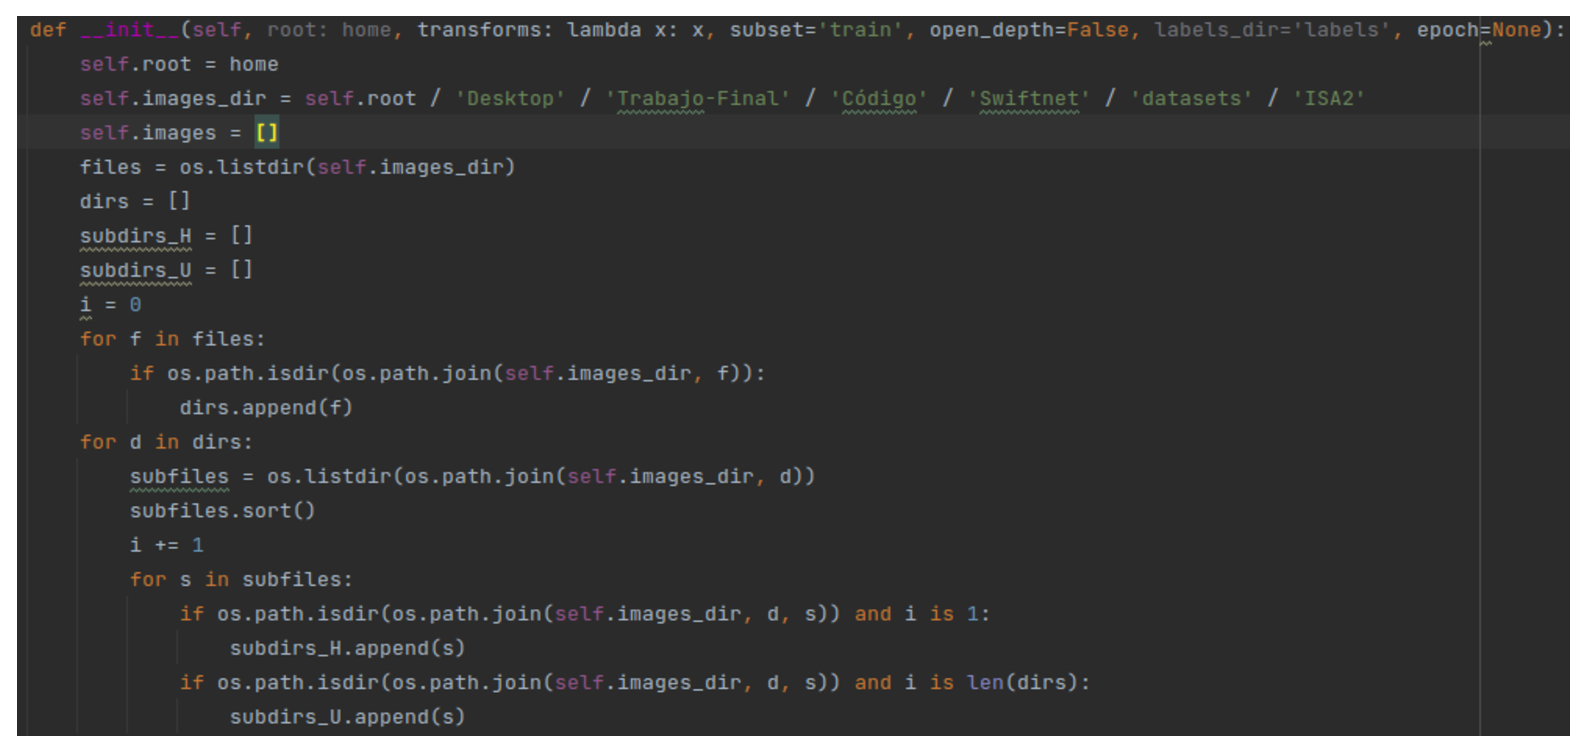
\includegraphics[width=16cm]{Figuras/cityscapes.py_1.eps}
  \caption{Archivo ``cityscapes.py'' Parte 1}
\end{figure}

\begin{figure}[H]
  \centering
  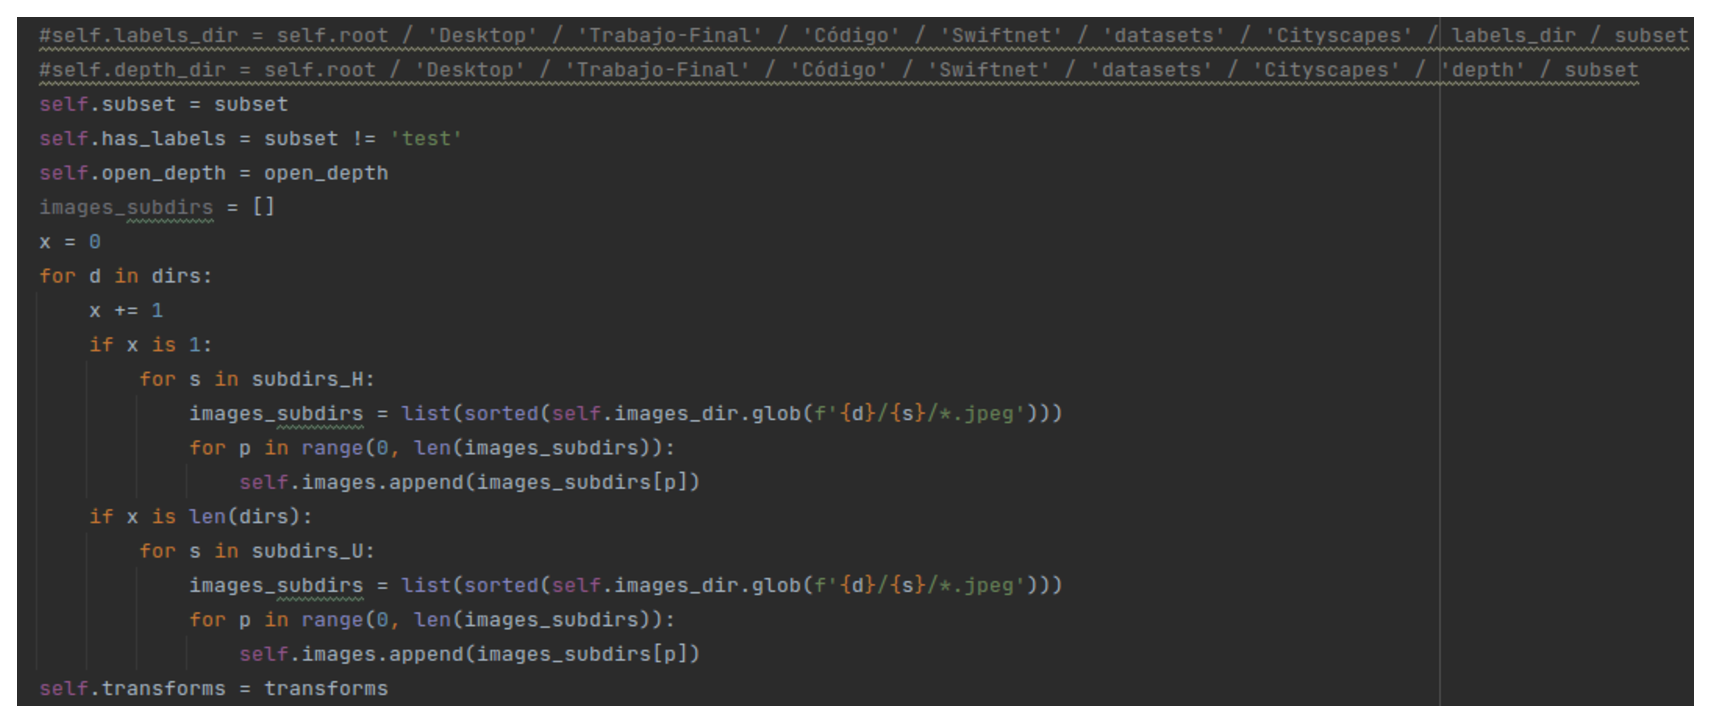
\includegraphics[width=16cm]{Figuras/cityscapes.py_2.eps}
  \caption{Archivo ``cityscapes.py'' Parte 2}
\end{figure}

\begin{figure}[H]
  \centering
  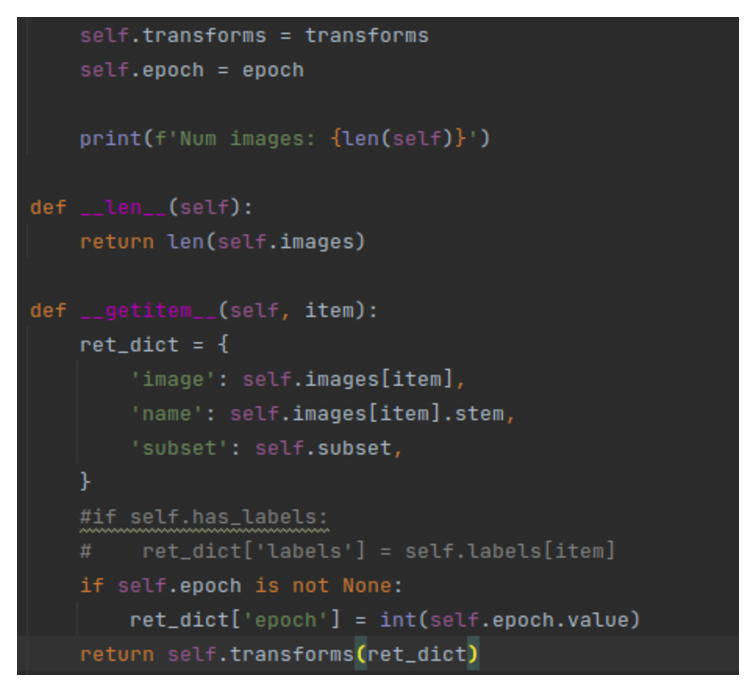
\includegraphics[width=8cm]{Figuras/cityscapes.py_3.eps}
  \caption{Archivo ``cityscapes.py'' Parte 3}
  \label{fig:pred.py3}
\end{figure}

\item Por último, modificar la clase ``StorePreds'' del archivo ``prediction.py'' en la carpeta ``evaluation\textbackslash{}'' siguiendo las siguientes figuras:

\begin{figure}[H]
  \centering
  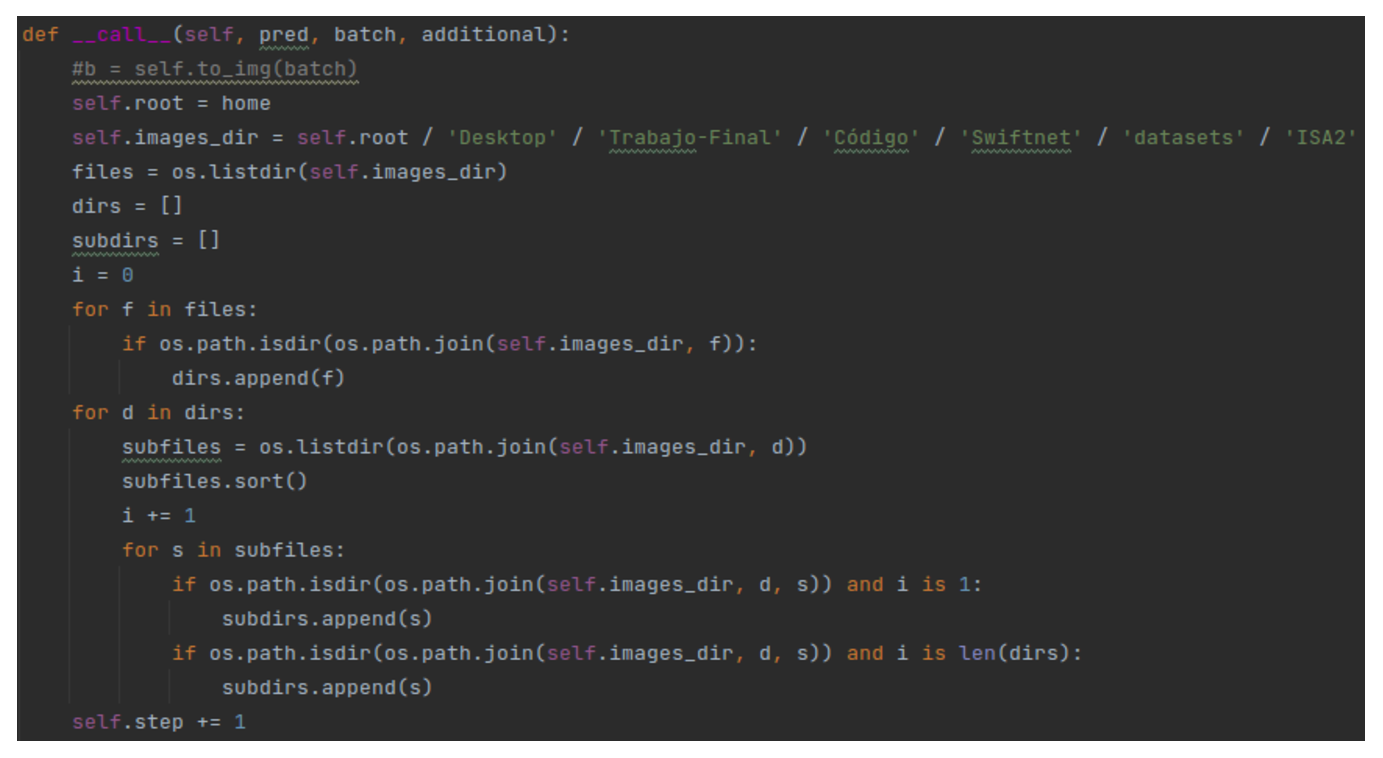
\includegraphics[width=16cm]{Figuras/prediction.py_1.eps}
  \caption{Archivo ``prediction.py'' Parte 1}
\end{figure}

\begin{figure}[H]
  \centering
  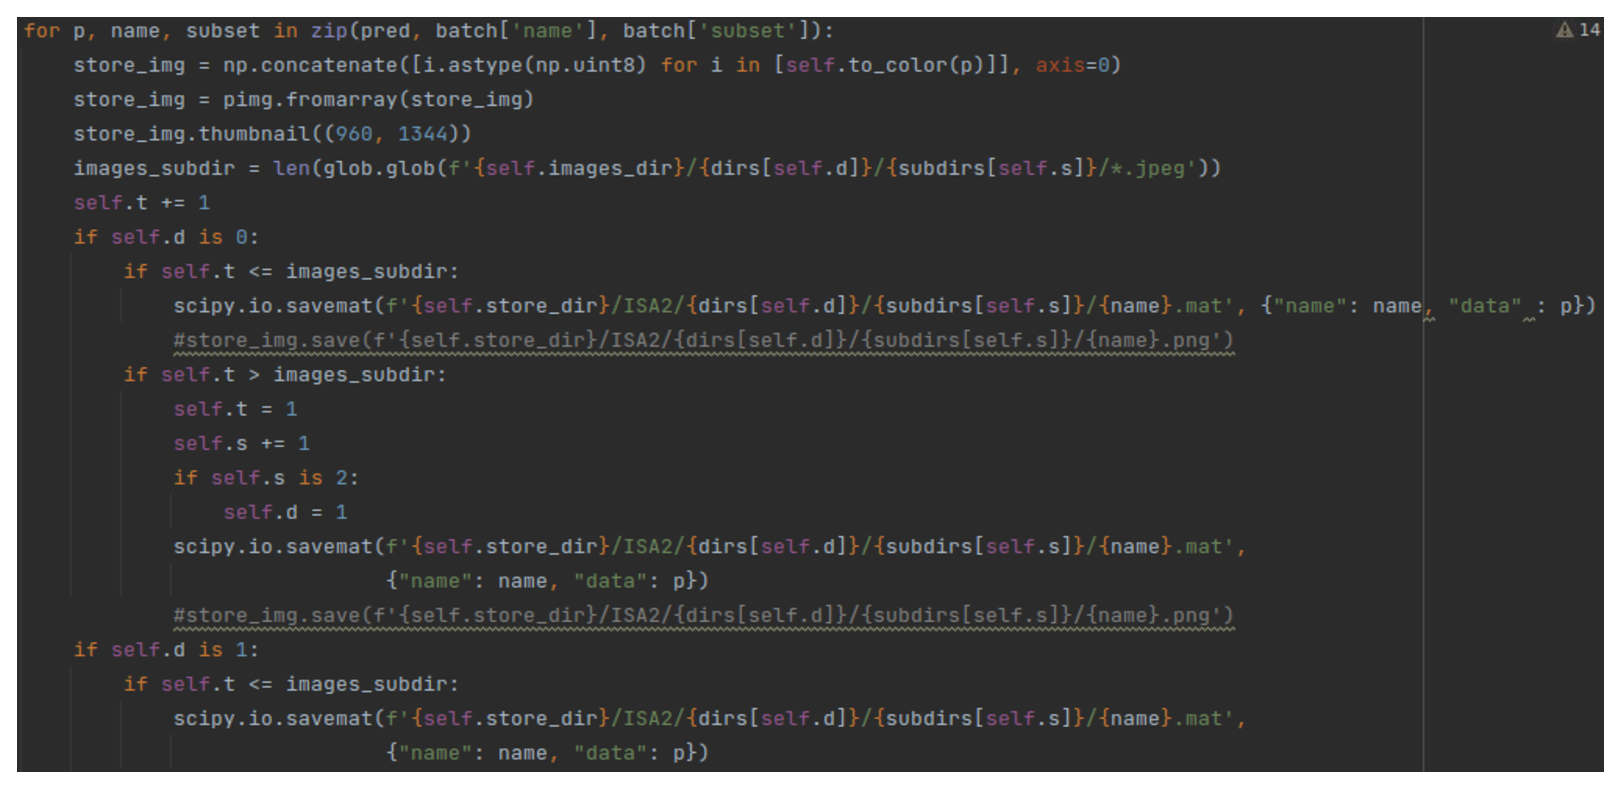
\includegraphics[width=16cm]{Figuras/prediction.py_2.eps}
  \caption{Archivo ``prediction.py'' Parte 2}
\end{figure}

\begin{figure}[H]
  \centering
  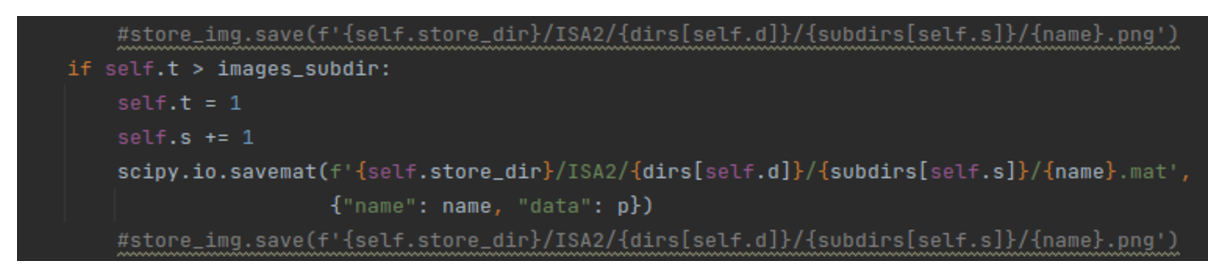
\includegraphics[width=16cm]{Figuras/prediction.py_3.eps}
  \caption{Archivo ``prediction.py'' Parte 3}
\end{figure}

Hemos modificado de esta manera el archivo ``cityscapes.py'' porque buscábamos que obtuviese las imágenes de manera automática de los subdirectorios de la base de datos de $ISA^{2}$. De la misma forma, los cambios en el archivo ``prediction.py'' persiguen el mismo objetivo: Guardar las imágenes procesadas de manera automática en los subdirectorios correspondientes.

A pesar de que son muchas modificaciones en estos dos últimos archivos, no son necesarias para la ejecución del modelo. En nuestro caso particular lo hemos hecho así por comodidad, pero no imprescindible para que funcione.

Siendo opcionales estas modificaciones, para lograr que el programa se ejecute con la base de datos de $ISA^{2}$ sin que se ``automatice'', basta con observar los mismos archivos para el dataset de Cityscapes y aplicar los cambios que se crean oportunos; ya que, teniéndolos como referencia, se puede ver de forma intuitiva qué partes se han de modificar. Sin embargo, la figura \ref{fig:pred.py3} es obligatoria en cualquier caso.

Cabe destacar que en el archivo ``prediction.py'', siguiendo las figuras, se puede ver la llamada a un método llamado ``savemat''. Éste sirve para guardar las imágenes segmentadas en archivos ``.mat'' que en el siguiente paso utilizaremos, de modo que, aunque no es estrictamente imprescindible, sí es recomendable usarlo puesto que nos resultará mucho más fácil manejar las imágenes segmentadas en los códigos de MatLab \cite{matlab} si están en ese formato.

\end{itemize}

Aquí acaba todo lo pertinente a Swiftnet. Hemos visto cómo ha segmentado las imágenes y el proceso interno que lo hace posible, además de trabajar con dos bases de datos. El siguiente paso es la realización de histogramas de las imágenes segmentadas y su posterior introducción en los sistemas de regresión para estimar la velocidad adecuada. Todo ello se hará en MatLab \cite{matlab}.

\section{Realización de histogramas}



\chapter{Resultados}

En la siguiente tabla pasamos a mostrar los resultados tanto de la versión anterior de $ISA^{2}$ como de la actual. Como ya dijimos anteriormente, el \ac{MAE} será la métrica que usaremos para esta tarea, pues indica cuánta precisión ha habido en la \ac{SS} realizada por el modelo Swiftnet \cite{swiftnet} con respecto al modelo DeepLab \cite{deeplab}.

Recordemos que, a raíz de la \ac{SS} realizada por uno de los modelos, generamos los histogramas que, posteriormente, se usaron en los sistemas de regresión para estimar la velocidad apropiada; de modo que el \ac{MAE} es una métrica muy acertada para saber qué versión del proyecto es mejor.

\begin{table}[H]
\centering
\resizebox{16cm}{!}{
\begin{tabular}{|l|l|l|l|l|l|}\cline{1-6}
& & \multicolumn{2}{|l|}{\textbf{MAE Swiftnet}} & \multicolumn{2}{|l|}{\textbf{MAE DeepLab}} \\ \cline{1-6}
\textbf{Regresión} & \textbf{Nivel de \ac{SPP}} & \textbf{Highway (\%)} & \textbf{Urban (\%)} & \textbf{Highway (\%)} & \textbf{Urban (\%)}\\ \cline{1-6}
\multirow{3}{*}{\textbf{\textit{Linear}}} & 1 & 12.22 & 8.95 & 10.32 & 8.38 \\ \cline{2-6}
& 2 & 13.94 & 9.45 & 11.18 & 8.81 \\ \cline{2-6}
& 3 & 13.39 & \textbf{\textit{11.79}} & 15.5 & \textbf{\textit{10.83}}\\ \cline{1-6}
\multirow{3}{*}{\textbf{\textit{Lasso}}} & 1 & 12.90 & 9.23 & 11.29 & 8.43 \\ \cline{2-6}
 & 2 & 13.80 & 9.40 & 11.7 & 8.62 \\ \cline{2-6}
 & 3 & 13.47 & 10.16 & 10.8 & 9.25\\ \cline{1-6}
\multirow{3}{*}{\textbf{\textit{Boosting Trees}}} & 1 & 13.43 & \textbf{9.83} & 11.35 & \textbf{10.14} \\ \cline{2-6}
 & 2 & 14.97 & \textbf{10.52} & 12.23 & \textbf{10.72}\\ \cline{2-6}
 & 3 & 14.75 & \textbf{10.08} & 10.37 & \textbf{10.12}\\ \cline{1-6}
\multirow{3}{*}{\textbf{\textit{SVR}}} & 1 & 11.13 & \textbf{8.74} & 9.69 & \textbf{9.55} \\ \cline{2-6}
 & 2 & 12.24 & \textbf{8.98} & 9.98 & \textbf{9.09}\\ \cline{2-6}
 & 3 & 12.09 & \textbf{9.60} & 9.78 & \textbf{9.62}\\ \cline{1-6}
\end{tabular}
}
\caption{Tabla de resultados}
\end{table}

Como se puede apreciar, para cada modelo de \ac{SS} se han segmentado imágenes correspondientes a autovías (o autopistas) y a entornos urbanos.

Los valores de Swiftnet que aparecen \textbf{resaltados de esta forma} indican que son mejores que los valores de DeepLab (\textbf{también resaltados}) para esa fila.

Por otro lado, hemos puesto dos valores con \textit{\textbf{este aspecto}} para indicar que, durante la predicción de la velocidad en el sistema de regresión lineal, hemos modificado un parámetro para obtener unos resultados más apropiados; ya que, de otra forma, se obtendrían valores muy lejanos a la realidad.

Como se puede observar, tanto los sistemas \textit{Boosting Trees} como \textit{\ac{SVR}} son mejores con la nueva versión para entornos urbanos, mientras que para las autovías es mejor utilizar el modelo DeepLab. Esto quiere decir que Swiftnet trabaja mejor con entornos en los que se requiere más nivel de detalle y DeepLab, por el contrario, lo realiza mejor en entornos más abiertos.

Cabe destacar que Swiftnet \cite{swiftnet} es un modelo \textbf{Real-Time}, de modo que su implementación es menos que costosa que DeepLab, el cual, por el contrario, necesita de un tiempo de procesamiento para realizar su función.

A continuación mostramos algunas figuras con las que podemos ver, de forma gráfica, los resultados de los sistemas de regresión con la \ac{SS} realizada por Swiftnet:

\begin{figure}[H]
  \centering
  \begin{subfigure}[b]{0.45\linewidth}
    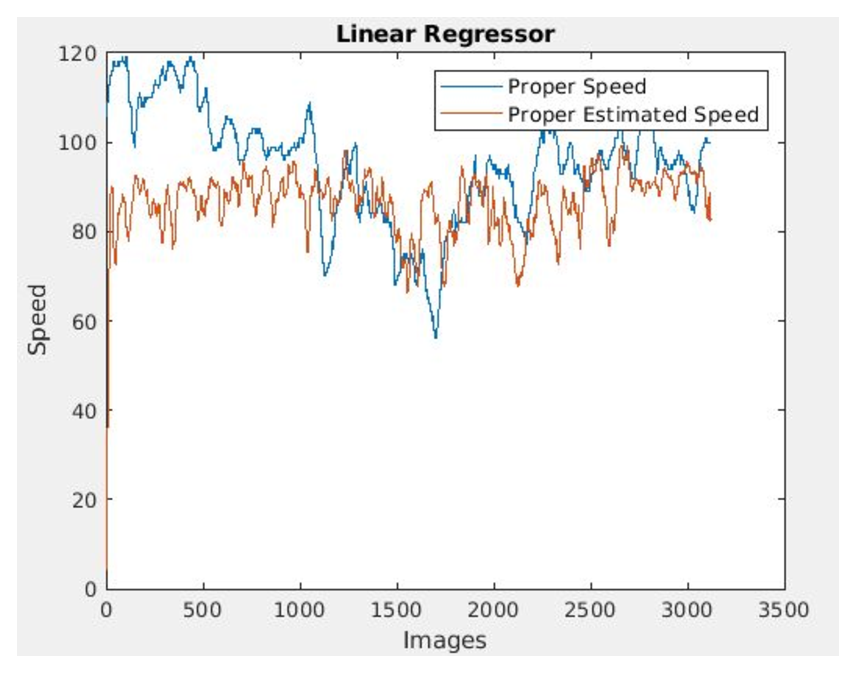
\includegraphics[width=\linewidth]{Figuras/Lineal_Highway(Nivel_1).eps}
    \caption{Highway con Lineal en nivel 1 de \ac{SPP}}
  \end{subfigure}
    \begin{subfigure}[b]{0.425\linewidth}
    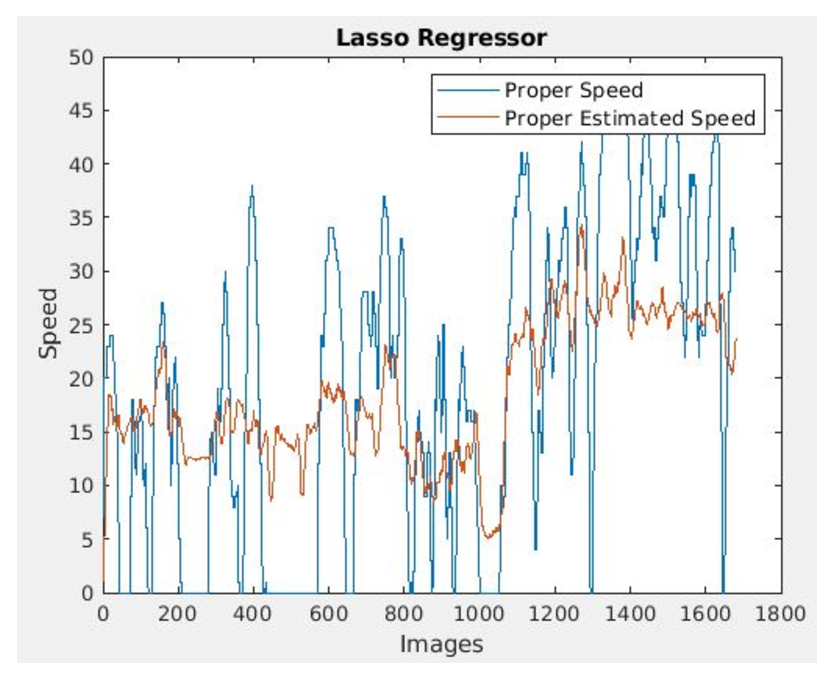
\includegraphics[width=\linewidth]{Figuras/Lasso_Urban(Nivel_1).eps}
    \caption{Urban con Lasso en nivel 1 de \ac{SPP}}
  \end{subfigure}
    \begin{subfigure}[b]{0.45\linewidth}
    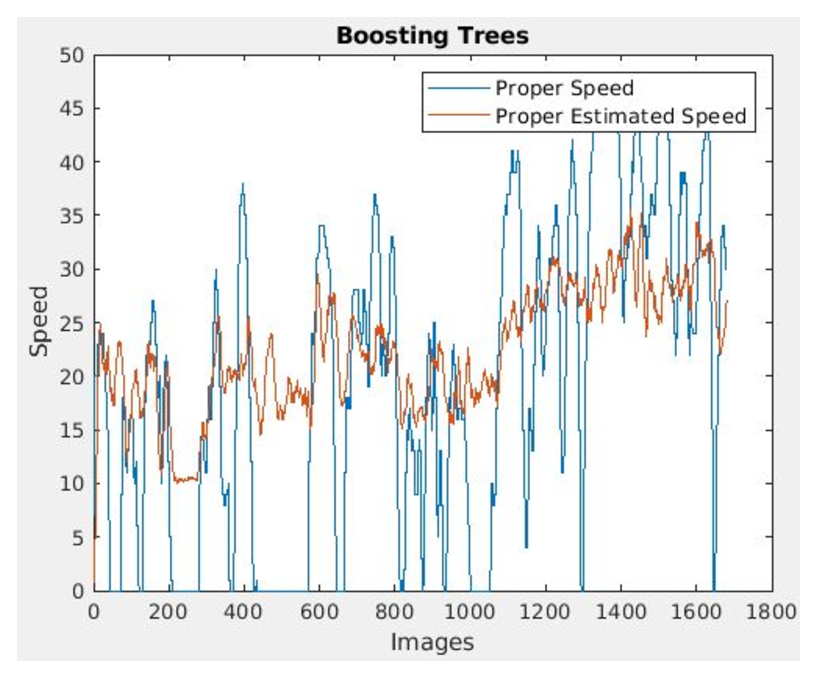
\includegraphics[width=\linewidth]{Figuras/Boosting_Urban(Nivel_1).eps}
    \caption{Urban con Boosting en nivel 1 de \ac{SPP}}
  \end{subfigure}
      \begin{subfigure}[b]{0.45\linewidth}
    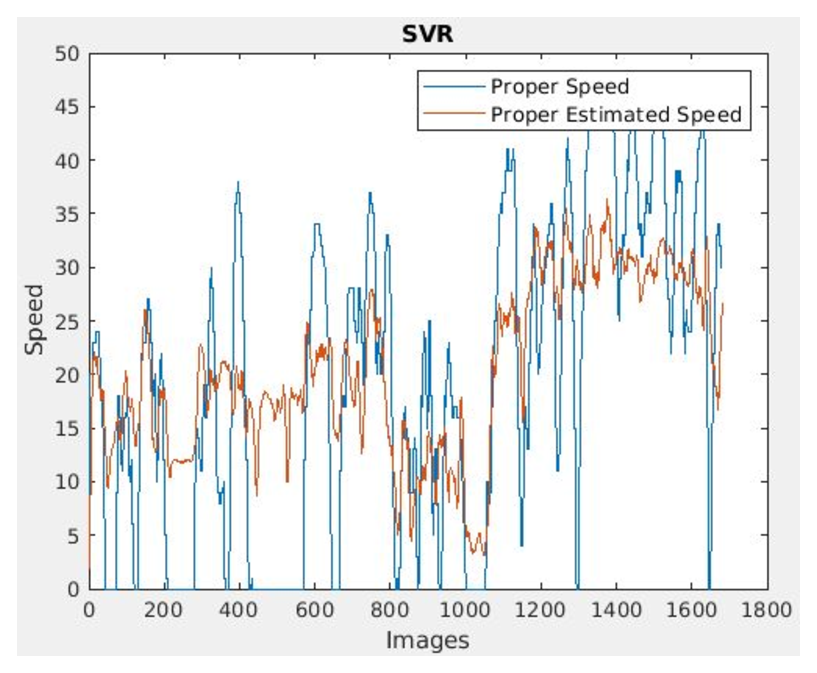
\includegraphics[width=\linewidth]{Figuras/SVR_Urban(Nivel_1).eps}
    \caption{Urban con SVR en nivel 1 de \ac{SPP}}
  \end{subfigure}
  \caption{Resultados gráficos}
\end{figure}

En las figuras, los puntos azules representan la velocidad \textbf{real} a la que debe ir el vehículo en cada imagen, mientras que los puntos rojos representan la velocidad \textbf{estimada} por los sistemas de regresión en cada imagen.

Como se puede observar, hemos escogido, en su mayoría, aquellas figuras en las que los sistemas de regresión han dado mejores resultados, es decir, en entornos urbanos \textbf{(Urban)}. Sin embargo, para contrastar cómo trabaja Swiftnet en autovías hemos decidido poner una figura con esos datos (\textbf{Highway}).

Hemos visto cómo se realiza todo el proceso de este trabajo y hemos comparado los resultados actuales con los anteriores. A continuación, finalizaremos con las conclusiones de éste.

\chapter{Conclusiones}

En este trabajo hemos contribuido a la evolución del sistema $ISA^{2}$ como respuesta a los sistemas \ac{ISA} ya existentes \cite{isa2}. Asimismo, hemos podido comprobar cómo al implementar un modelo \textbf{Real-Time} con una mayor precisión para la \ac{SS} (Swiftnet \cite{swiftnet}), el propio sistema mejora en aspectos muy importantes:

\begin{itemize}
\item Mayor precisión en entornos urbanos.
\item Menor coste de implementación.
\item Mayor velocidad de procesado de imágenes para realizar la \ac{SS}.
\end{itemize}

De modo que, usando este modelo, con las variaciones que ello conlleva, podemos asegurar que este sistema es mejor que su predecesor.

Por todo ello, concluimos con la idea de que esta nueva versión de $ISA^{2}$ sirva como punto de referencia para futuras mejoras del mismo. Al principio de este trabajo, contamos cómo con los sistemas \ac{ISA}, se habían reducido cuantiosamente el número de accidentes de tráfico en España... Con este sistema, y con los que se deriven de éste, esperemos que, en un futuro no muy lejano, ese dato no exista.


%Prepara la sección de apéncices, si es que se necesita.
%\appendix
%% Formato para un capítulo cualquiera

%Título del capítulo
\chapter{CÓDIGO FUENTE.} 
%Sección primera
\section{Primera sección del apéndice.}
Texto de la primera sección.
\subsection{Segunda sección del apéndice.}
Texto de la segunda sección.
\subsubsection{Tercera sección del apéndice.}
Texto de la tercera sección.

%\include{fichero-apendice-b}


\backmatter

\nocite{*}



%*****************************
%Sección para la bibliografía
%*****************************

%Posibles estilos de bibliografia
\bibliographystyle{plain}
%\bibliographystyle{abbrvnat}
%\bibliographystyle{klunamed}
%\bibliographystyle{unsrt}

\addcontentsline{toc}{chapter}{{}Bibliografía}

%Toma los datos del fichero bibliografia-pfc.bib
\bibliography{bibliografia-pfc}

%\printindex

\end{document}

%Final de la plantilla.